%Struktur: 20 min Vortrag mit 1,5 min pro Folie -> 15 Folien inkl. Titelfolie
%10 min Fragen

%%%%%%%%%%%%%%%%%%%%%%%%%%%%%%%%%%%%%%%%%%%%%%%%%%%%%%%%%%%%%%%%%%%%%%%%%%%%%%%%%%%%%%%%%%%%%%%%%%%%%%%%%%%%%%%%%%%%%%%%%%%%%%%%%%%%%%

\documentclass[colorbacktitle,inverttitle,landscape,presentation,
	english,
	aspectratio=43, %43 or 169, 1610
	accentcolor=tud9b, %tud9b (temf) or tud5b (gsce) 
]{tudbeamer}

%%additional packages(Praesentation)
%%standard:

%%language:
\usepackage[utf8]{inputenc}
\usepackage[english]{babel}
%%math:
\usepackage{amsmath}
\usepackage{caption}
\usepackage{subcaption}
%%tikz:
\usepackage{tikz}
\usetikzlibrary{patterns}
\usepackage[siunitx,americaninductors]{circuitikz}
\usepackage{siunitx}
%%pgfplots:
\usepackage{pgfplots}
\usepgfplotslibrary{groupplots}
\usepgfplotslibrary{patchplots}
\usepackage{pgfplotstable}
\pgfplotsset{compat=newest}\usepgfplotslibrary{units}
%%scaling:
\usepackage{adjustbox}
\usepackage{wrapfig,lipsum,booktabs}
%%additional packages(Praesentation)
 

%needs to come last
\usepackage{temfbeamer}

%remove TU logo from every slide but the title
\setbeamertemplate{headline}[TUD theme nologo] 

\definecolor{mygreen}{rgb}{0,0.6,0}
\definecolor{mygray}{rgb}{0.5,0.5,0.5}
\definecolor{mymauve}{rgb}{0.58,0,0.82}
\usepackage{listings}
\lstset{ %
  float=tp,
  floatplacement=tbp,
  abovecaptionskip=-5pt,
  backgroundcolor=\color{gray!25},   % choose the background color; you must add \usepackage{color} or \usepackage{xcolor}; should come as last argument
  basicstyle=\scriptsize,        % the size of the fonts that are used for the code
  breakatwhitespace=false,         % sets if automatic breaks should only happen at whitespace
  breaklines=true,                 % sets automatic line breaking
  commentstyle=\color{mygreen},    % comment style
  frame=single,	                   % adds a frame around the code
  keepspaces=true,                 % keeps spaces in text, useful for keeping indentation of code (possibly needs columns=flexible)
  keywordstyle=\color{blue},       % keyword style
  language=Python,                 % the language of the code
%  morekeywords={*,...},            % if you want to add more keywords to the set
  numbers=left,                    % where to put the line-numbers; possible values are (none, left, right)
  numbersep=5pt,                   % how far the line-numbers are from the code
  numberstyle=\tiny\color{mygray}, % the style that is used for the line-numbers
  rulecolor=\color{black},         % if not set, the frame-color may be changed on line-breaks within not-black text (e.g. comments (green here))
  showspaces=false,                % show spaces everywhere adding particular underscores; it overrides 'showstringspaces'
  showstringspaces=false,          % underline spaces within strings only
  showtabs=false,                  % show tabs within strings adding particular underscores
  stepnumber=1,                    % the step between two line-numbers. If it's 1, each line will be numbered
  stringstyle=\color{mymauve},     % string literal style
  tabsize=2,	                   % sets default tabsize to 2 spaces
}

\usepackage[absolute,overlay]{textpos}
 
 
  \setlength{\TPHorizModule}{1mm}
  \setlength{\TPVertModule}{1mm}

%set date
\date{13. August, 2018}

\newcount\WertA

\newcounter{from}
\newcounter{till}
\newcounter{onlyAt}

%%%%%%%%%%%%%%%%%%%%%%%%%%%%%%%%%%%%%%%%%%%%%%%%%%%%%%%%%%%%%%%%%%%%%%%%%%%%%%%%%%%%%%%%%%%%%%%%%%%%%%%%%%%%%%%%%%%%%%%%%%%%%%%%%%%%%%

\title{Generierung des Eingangssingals für Barrier Bucket RF Systeme and der GSI }

\subtitle{\\[0.3\baselineskip]
	Jonas Christ, Artem Moskalew, Maximilian Nolte \\
{\small Jens Harzheim, M.Sc.}\\
[0.3\baselineskip]
{\tiny Projektseminar Beschleunigertechnik}\\[0.3em]
	\mbox{\scriptsize}~}
	
\institute[TU Darmstadt | Fachbereich 18 | Institut Theorie Elektromagnetischer Felder]{Institut für Theorie Elektromagnetischer Felder, TU Darmstadt}

%%%%%%%%%%%%%%%%%%%%%%%%%%%%%%%%%%%%%%%%%%%%%%%%%%%%%%%%%%%%%%%%%%%%%%%%%%%%%%%%%%%%%%%%%%%%%%%%%%%%%%%%%%%%%%%%%%%%%%%%%%%%%%%%%%%%%%



\begin{document}
	
\begin{titleframe}
	\tudtitle[images/temf_logo.pdf]{images/temf_background.jpg} 
	%\tudtitle[images/gsce_logo.pdf]{images/gsce_background.jpg}
	\end{titleframe}
	
\begin{frame}
	\frametitle{Outline}
	\tableofcontents%[currentsection,subsectionstyle=show/show/hide]
\end{frame}
	
%%%%%%%%%%%%%%%%%%%%%%%%%%%%%%%%%%%%%%%%%%%%%%%%%%%%%%%%%%%%%%%%%%%%%%%%%%%%%%%%%%%%%%%%%%%%%%%%%%%%%%%%%%%%%%%%%%%%%%%%%%%%%%%%%%%%%%

\section{Einführung}

\subsection{Problemstellung}
\begin{frame}{Problemstellung}

\end{frame}





\subsection{Aufbau}
\begin{frame}[fragile]
\frametitle{Aufbau und Modell}

\begin{center}
		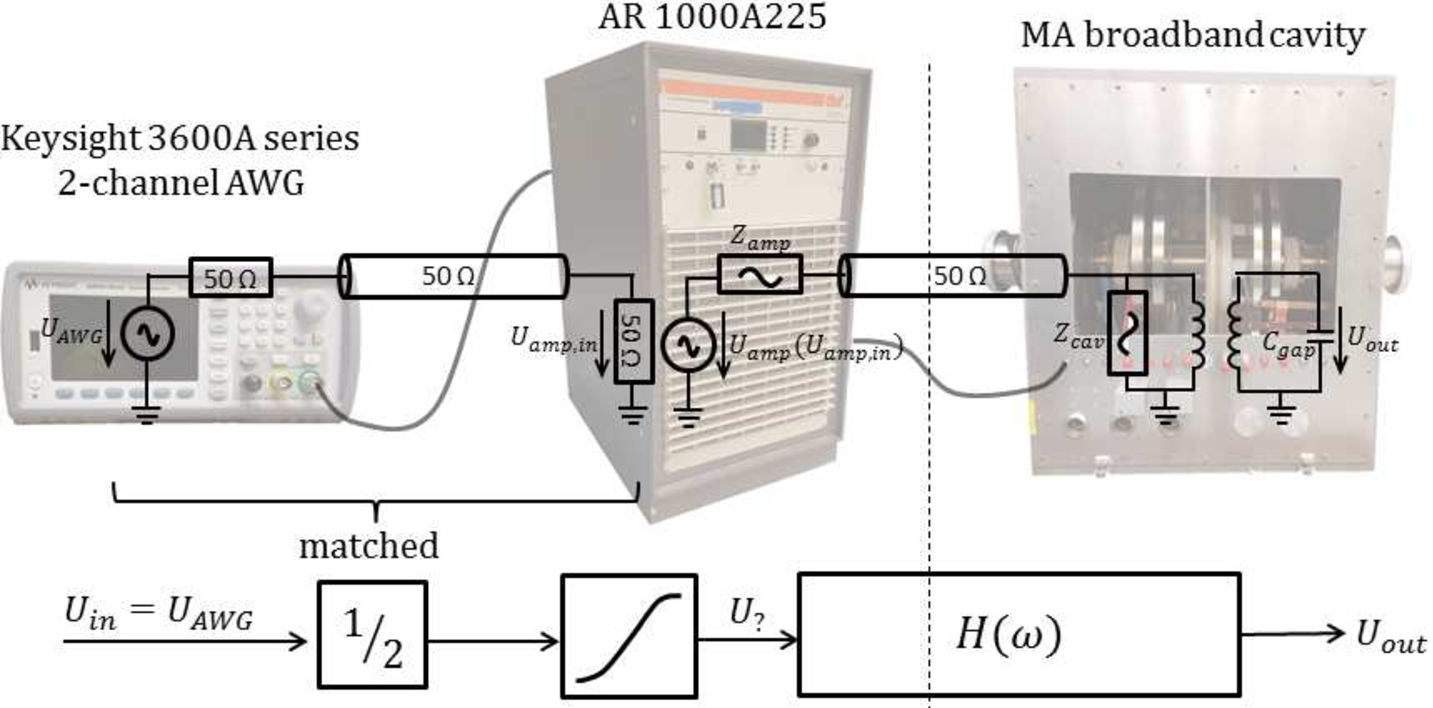
\includegraphics[scale=0.45]{slides/ResultCode/WEPVA047f2_2-eps-converted-to.pdf} 
	\end{center}
\end{frame}

\begin{frame}[fragile]
\frametitle{Aufbau und Modell}

	
	{
	\begin{itemize}
	\uncover<2->{
	\item Gegeben:
		\begin{itemize} 
			\item Lineare Übertragungsfunktion $H$ bestimmt durch Pseudorauschen
			\item System linear bis $\hat{U}_{BB} \approx 550V$ genähert
		\end{itemize}
		}
		\uncover<3->{
	\item Hammerstein Modell : 
		\begin{itemize}
			\item Ergänzung um eine nichtlineare Vorverzerrung mit einem Potenzreihenansatz 
		\end{itemize}
		\begin{center}
		%\begin{align*}
		$	U_?(t)=\sum_{n=1}^N \, a_n \, \left[ U_{in}(t) \right]^n
			\quad
			\underline{U}_{out} \left( \omega \right) = H \left( \omega \right) \cdot \underline{U}_{?} \left( \omega \right)
		$\\		
		%\end{align*}
		}
		\end{center}
		\uncover<4->{
	\item Zielsetzung :
		\begin{itemize}
			\item Parameter $a_n$ der Kennlinie $K$ zubestimmen
			\item Ersten Optimierungs Ansatz implementieren
		\end{itemize}
		}	
	 \end{itemize}
	
	\centering
	\begin{picture}(100,70)
		\put(15,5){
			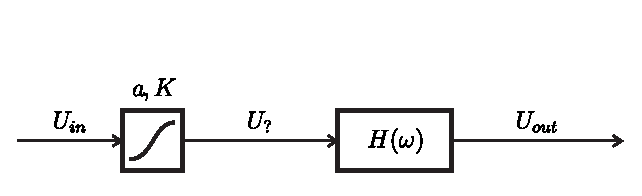
\includegraphics[scale=1.0]{slides/Problemstellung/Slide1.eps} 
		}
	\end{picture}
	}
%\begin{picture}(100,70)
%		\put(15,0){
%			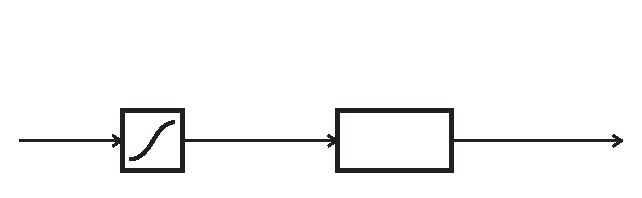
\includegraphics[scale=1.0]{slides/ResultCode/Slide2.eps} 
%		}  
%	\end{picture}
\end{frame}



%\section{Code}

%\WertA=1
%\subsection{Design}
%

\begin{frame}[fragile]
\ifnum\WertA=1
\frametitle{Code: Das Design}
\else
\frametitle{Code: Evaluierung}
\fi

%\only<1>
%	{ 
%\framebox{   %   % just so you can see where the "picture" is

\setcounter{onlyAt}{0}

\ifnum\WertA=1

%\setcounter{onlyAt}{\value{onlyAt}+1}
%\only<\value{onlyAt}>
%{
%	\begin{center}
%		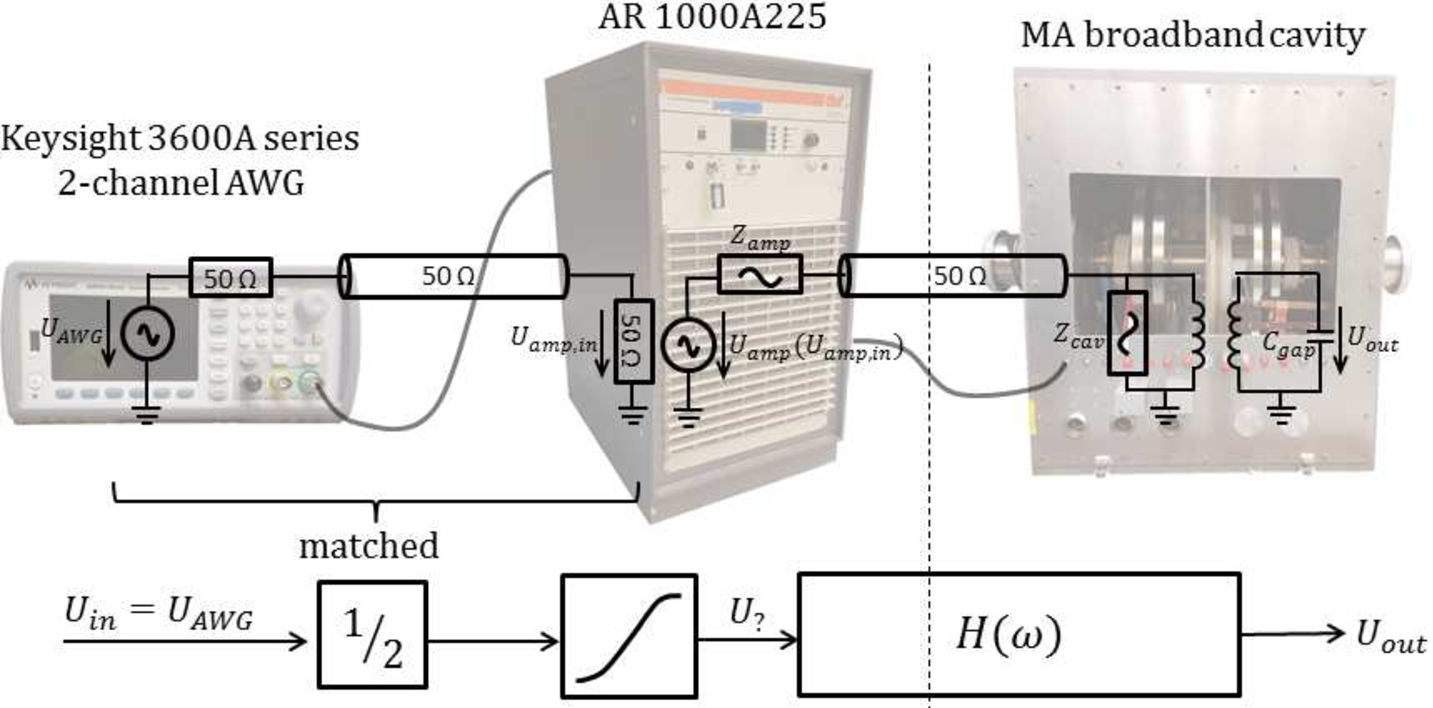
\includegraphics[scale=0.45]{slides/ResultCode/WEPVA047f2_2-eps-converted-to.pdf} 
%	\end{center}
%}

\setcounter{onlyAt}{\value{onlyAt}+1}
\only<\value{onlyAt}>
	{
	\begin{picture}(100,70)
		\put(15,0){
			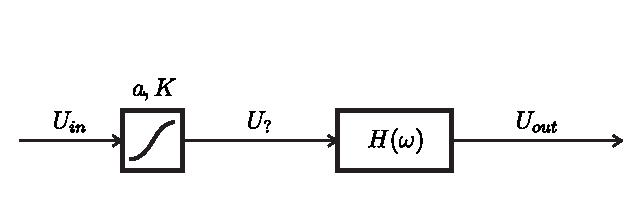
\includegraphics[scale=1.0]{slides/ResultCode/Slide1.eps} 
		}  
	\end{picture} 
	}
\fi
		
\setcounter{onlyAt}{\value{onlyAt}+1}
\only<\value{onlyAt}>
	{
	\begin{picture}(100,70)
		\put(15,0){
			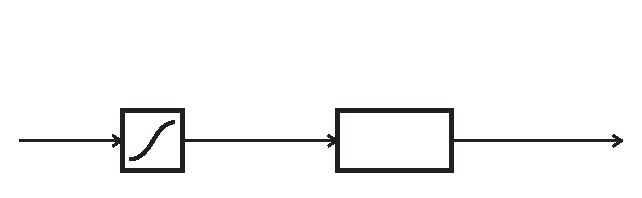
\includegraphics[scale=1.0]{slides/ResultCode/Slide2.eps} 
		}  
	\end{picture} 
	}
	


\ifnum\WertA=1 \setcounter{from}{\value{onlyAt}+1} \setcounter{till}{\value{onlyAt}+1} \else \setcounter{from}{\value{onlyAt}+1} \setcounter{till}{\value{onlyAt}+2} \fi	
\only<\value{from} - \value{till}> 
	{
	\begin{picture}(100,70)
		\put(15,0){
			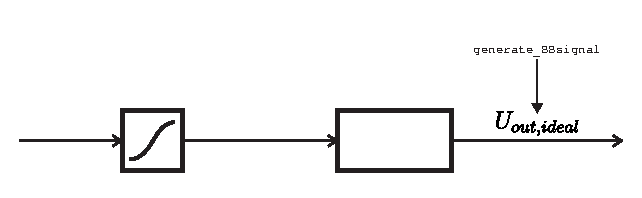
\includegraphics[scale=1.0]{slides/ResultCode/Slide3.eps} 
		}  
	\end{picture} 
	\lstinputlisting[firstline=1,lastline=1]{slides/ResultCode/file.txt} 
	}	
	
\ifnum\WertA=2
	\setcounter{onlyAt}{\value{from} + 1}
	\only<\value{onlyAt}>
	{
		\begin{textblock}{20}(80,50)
    		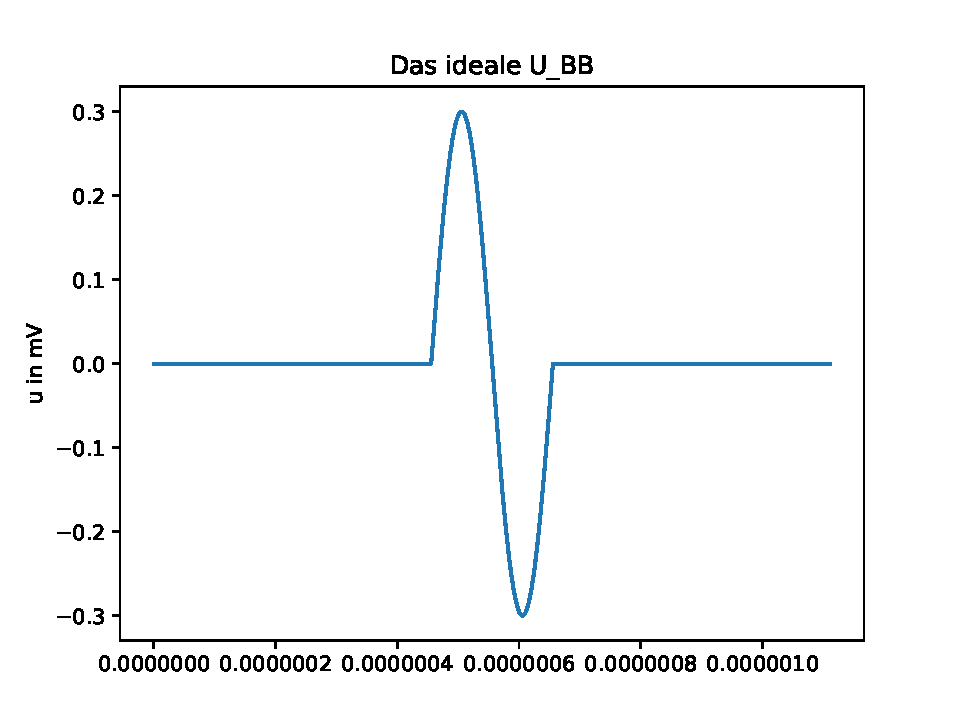
\includegraphics[height=3.5cm, width=4.5cm ]{slides/ResultCode/plots/Uout_ideal.pdf} 
		\end{textblock}	
	} 	
\fi	
\setcounter{onlyAt}{\value{till}}


\ifnum\WertA=1 \setcounter{from}{\value{onlyAt}+1} \setcounter{till}{\value{onlyAt}+1} \else \setcounter{from}{\value{onlyAt}+1} \setcounter{till}{\value{onlyAt}+2} \fi	
\only<\value{from} - \value{till}> 
	{
	\begin{picture}(100,70)
		\put(15,0){
			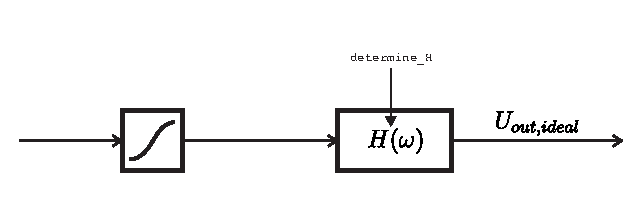
\includegraphics[scale=1.0]{slides/ResultCode/Slide4.eps} 
		}  
	\end{picture} 
	\lstinputlisting[firstline=1,lastline=2]{slides/ResultCode/file.txt} 
	}
	
\ifnum\WertA=2
	\setcounter{onlyAt}{\value{from} + 1}
	\only<\value{onlyAt}>
	{
		\begin{textblock}{20}(93,50)
    		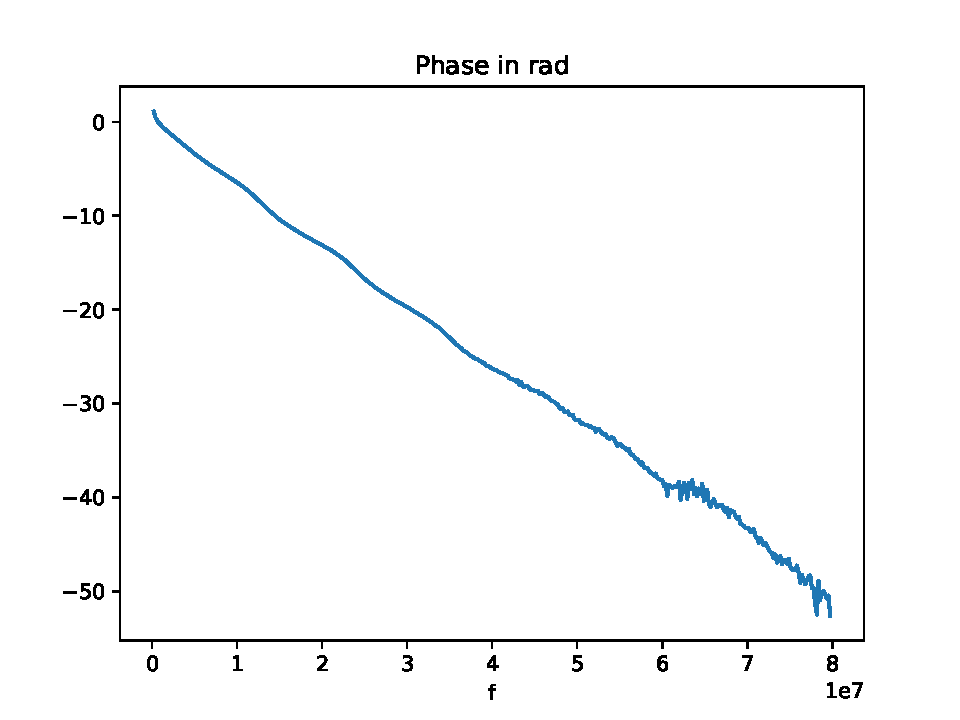
\includegraphics[ width=3.5cm, height=3.1cm ]{slides/ResultCode/plots/H_p.pdf} 
		\end{textblock}			
		\begin{textblock}{20}(61,50)
    		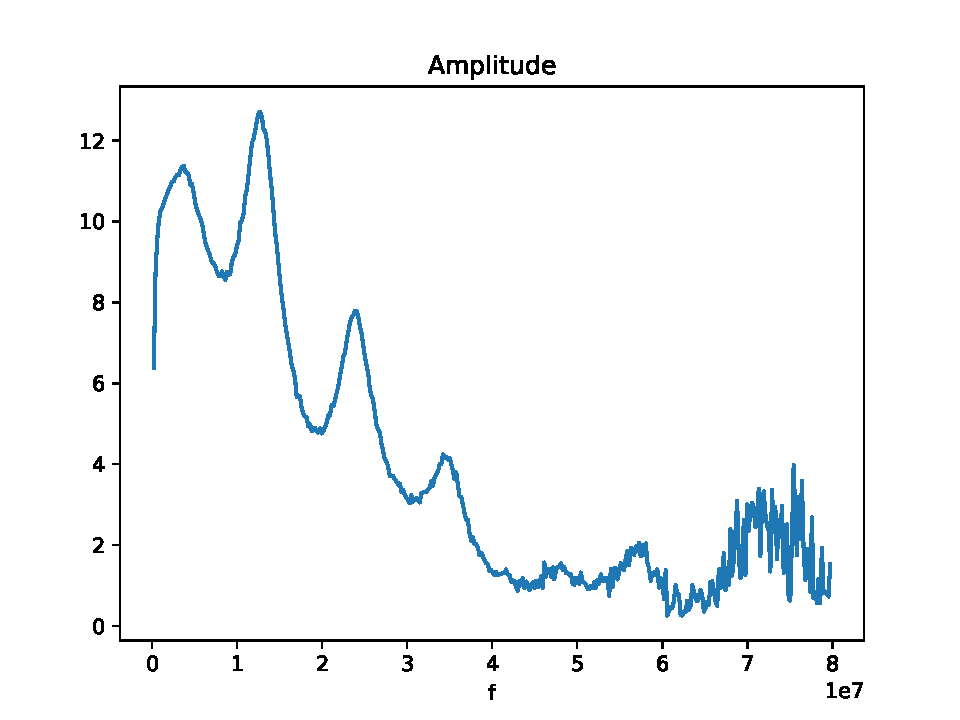
\includegraphics[ width=3.5cm, height=3.1cm]{slides/ResultCode/plots/H_a.pdf} 
		\end{textblock}	
		
	} 	 
\fi	
\setcounter{onlyAt}{\value{till}} 

\setcounter{onlyAt}{\value{onlyAt}+1}
\only<\value{onlyAt}>
	{
	\begin{picture}(100,70)
		\put(15,0){
			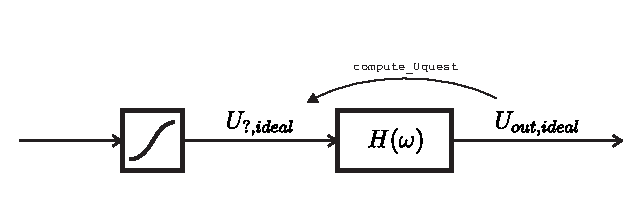
\includegraphics[scale=1.0]{slides/ResultCode/Slide5.eps} 
		}  
	\end{picture} 
	\lstinputlisting[firstline=1,lastline=3]{slides/ResultCode/file.txt} 
	}	
	
\setcounter{onlyAt}{\value{onlyAt}+1}
\only<\value{onlyAt}>
	{
	\begin{picture}(100,70)
		\put(15,0){
			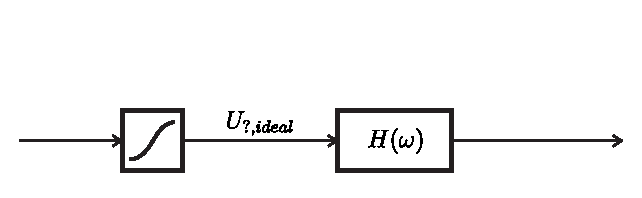
\includegraphics[scale=1.0]{slides/ResultCode/Slide5-1.eps} 
		}  
	\end{picture} 
	\lstinputlisting[firstline=1,lastline=3]{slides/ResultCode/file.txt} 
	}
	
\ifnum\WertA=2
	\setcounter{from}{\value{onlyAt}} 
	\setcounter{till}{\value{onlyAt}+2}
	\only<\value{from} - \value{till}>
	{
		\begin{textblock}{20}(80,50)
    		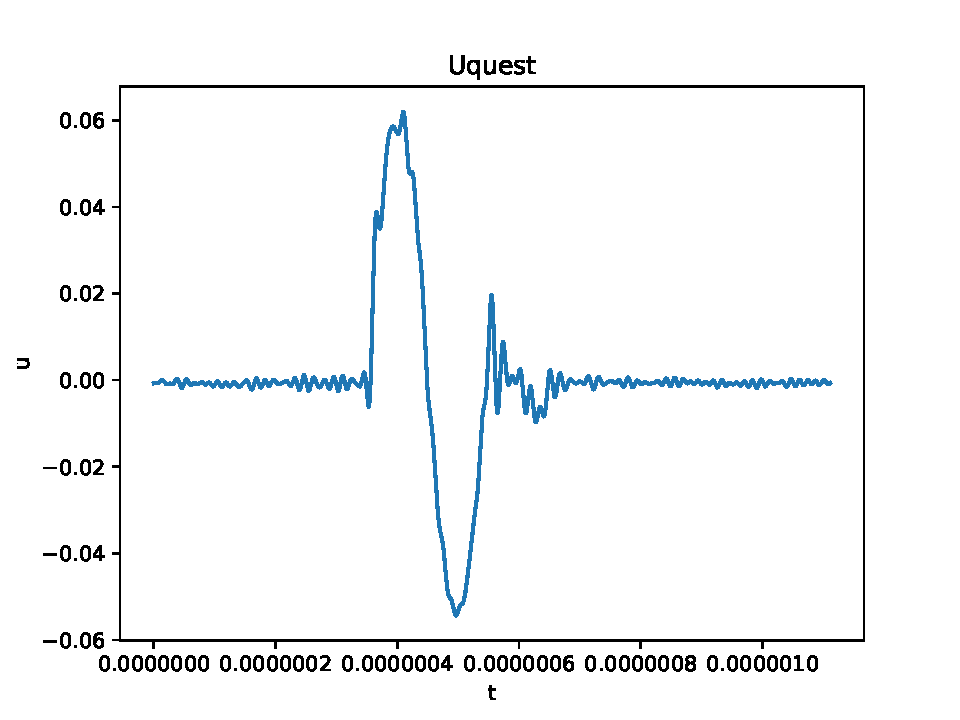
\includegraphics[height=3.5cm, width=4.5cm ]{slides/ResultCode/plots/U_quest_ideal.pdf} 
		\end{textblock}	
	} 
\fi	

\setcounter{onlyAt}{\value{onlyAt}+1}
\only<\value{onlyAt}>
{
	\begin{picture}(100,70)
		\put(15,0)
		{
			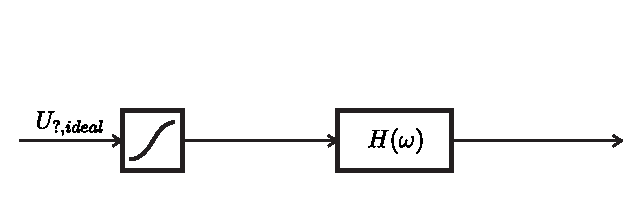
\includegraphics[scale=1.0]{slides/ResultCode/Slide6.eps} 
		}  
	\end{picture} 
	\lstinputlisting[firstline=1,lastline=3]{slides/ResultCode/file.txt} 
}

\setcounter{onlyAt}{\value{onlyAt}+1}
\only<\value{onlyAt}>
{
	\begin{picture}(100,70)
		\put(15,0)
		{
			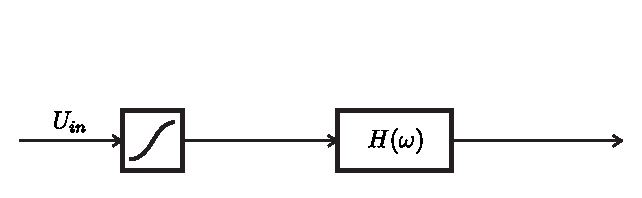
\includegraphics[scale=1.0]{slides/ResultCode/Slide7.eps} 
		}
	\end{picture} 	
	\lstinputlisting[firstline=1,lastline=4]{slides/ResultCode/file.txt} 	
}	

\setcounter{onlyAt}{\value{onlyAt}+1}
\only<\value{onlyAt}>
{
	\begin{picture}(100,70)
		\put(15,0)
		{
			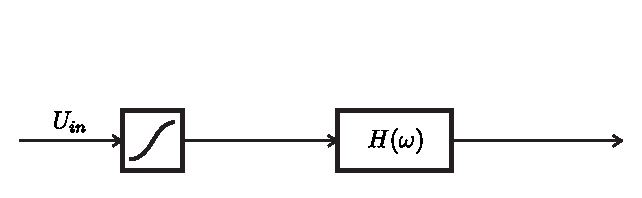
\includegraphics[scale=1.0]{slides/ResultCode/Slide7.eps} 
		}
	\end{picture} 	
	\lstinputlisting[firstline=1,lastline=5]{slides/ResultCode/file.txt} 		

}

\ifnum\WertA=1 \setcounter{from}{\value{onlyAt}+1} \setcounter{till}{\value{onlyAt}+1} \else \setcounter{from}{\value{onlyAt}+1} \setcounter{till}{\value{onlyAt}+3} \fi	
\only<\value{from} - \value{till}> 
{
	\begin{picture}(100,70)
		\put(15,0)
		{
			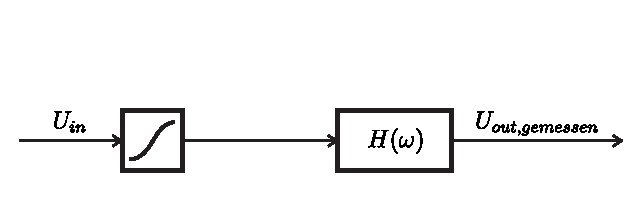
\includegraphics[scale=1.0]{slides/ResultCode/Slide8.eps} 
		}
	\end{picture} 	
	\lstinputlisting[firstline=1,lastline=5]{slides/ResultCode/file.txt} 		

}

\ifnum\WertA=2
	\setcounter{onlyAt}{\value{from}+1}
	\only<\value{onlyAt}>
	{
		\begin{textblock}{20}(80,50)
    		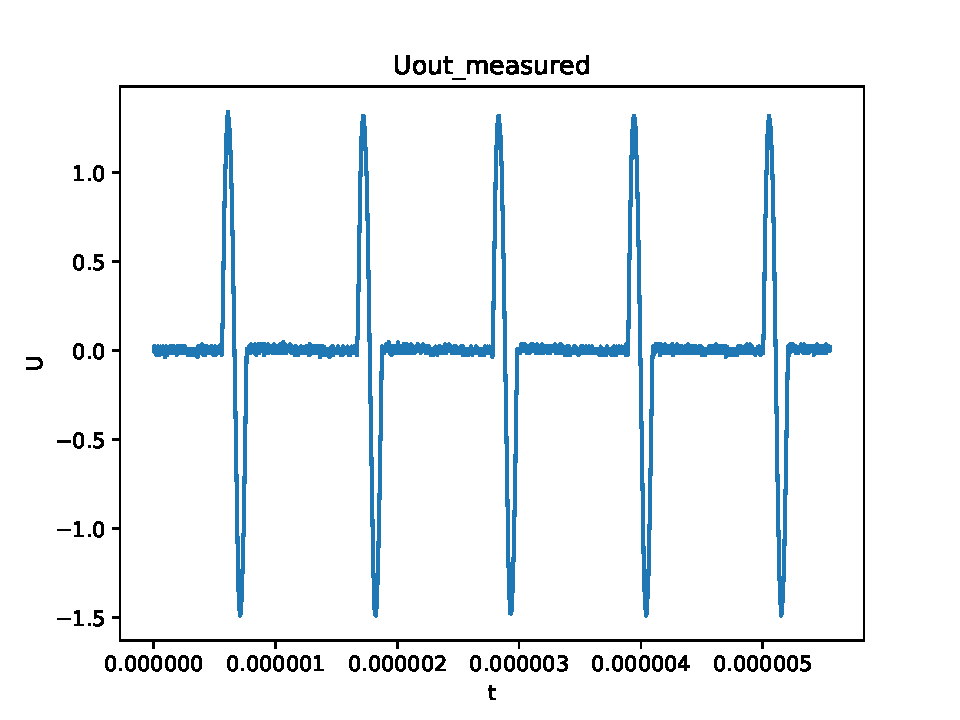
\includegraphics[height=3.5cm, width=4.5cm ]{slides/ResultCode/plots/Uout_measured.pdf} 
		\end{textblock}	
	} 
	\setcounter{onlyAt}{\value{from}+2}
	\only<\value{onlyAt}>
	{
		\begin{textblock}{20}(80,50)
    		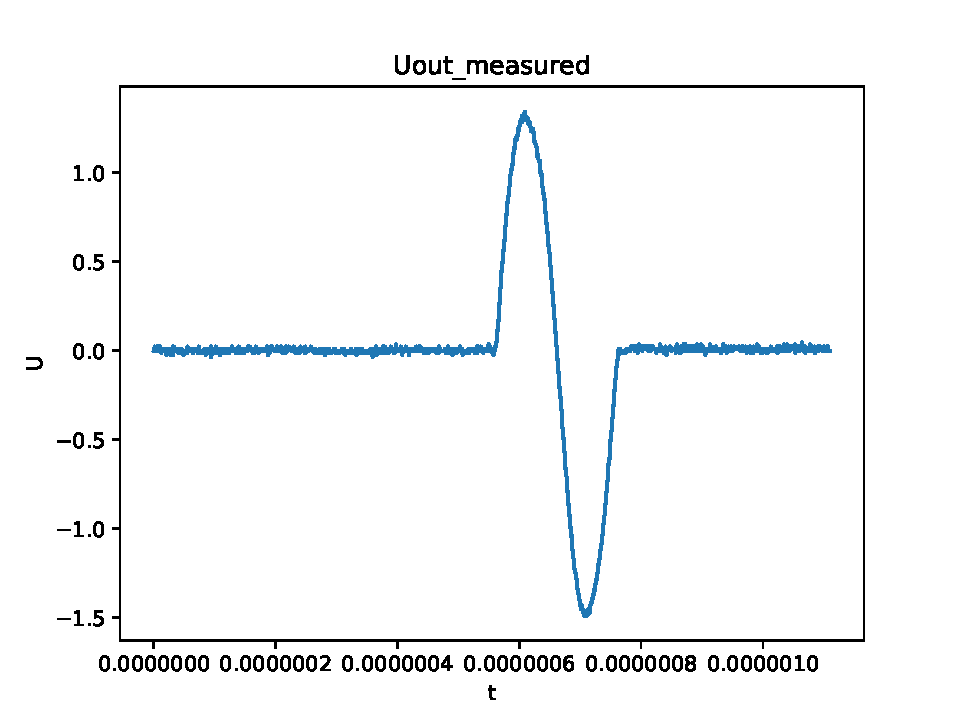
\includegraphics[height=3.5cm, width=4.5cm ]{slides/ResultCode/plots/Uout_measured_cut.pdf} 
		\end{textblock}	
	} 
\fi
\setcounter{onlyAt}{\value{till}} 
 
\ifnum\WertA=1 \setcounter{from}{\value{onlyAt}+1} \setcounter{till}{\value{onlyAt}+1} \else \setcounter{from}{\value{onlyAt}+1} \setcounter{till}{\value{onlyAt}+2} \fi	
\only<\value{from} - \value{till}> 
{
	\begin{picture}(100,70)
		\put(15,0)
		{
			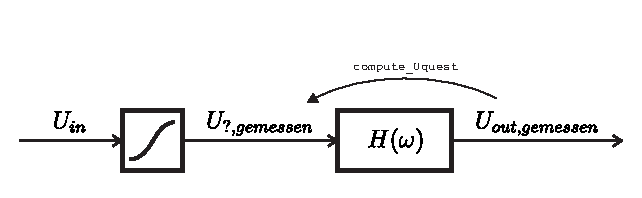
\includegraphics[scale=1.0]{slides/ResultCode/Slide9.eps} 
		}  
	\end{picture} 
	\lstinputlisting[firstline=1,lastline=6]{slides/ResultCode/file.txt} 
}	

\ifnum\WertA=2
	\setcounter{onlyAt}{\value{from} + 1}
	\only<\value{onlyAt}>
	{
		\begin{textblock}{20}(80,50)
    		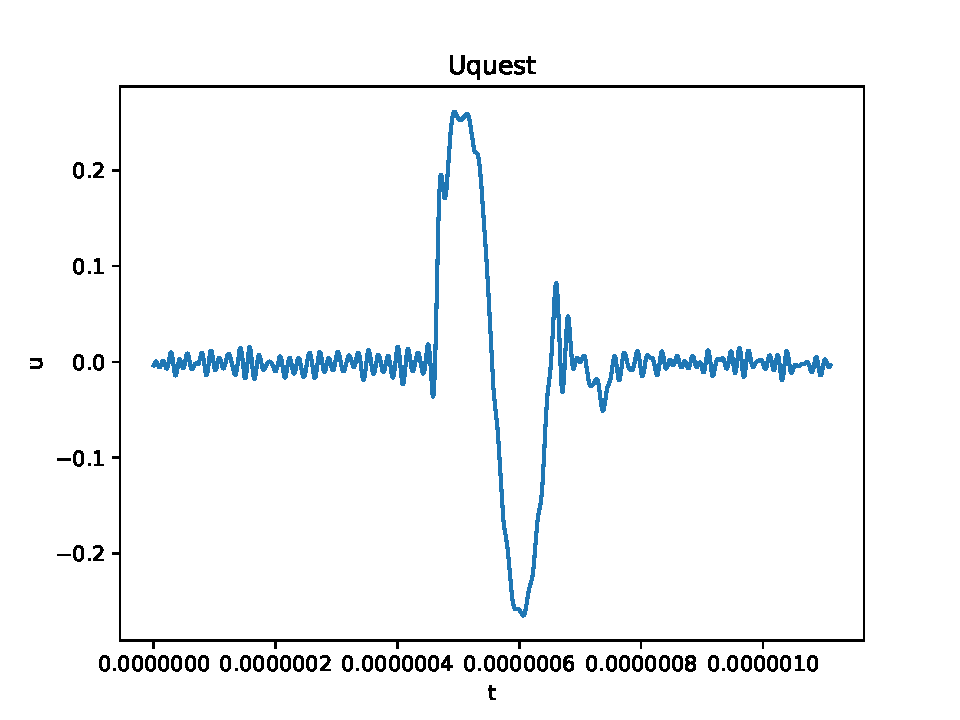
\includegraphics[height=3.5cm, width=4.5cm ]{slides/ResultCode/plots/U_quest_measured.pdf} 
		\end{textblock}	
	}
\fi
\setcounter{onlyAt}{\value{till}} 
	
\ifnum\WertA=1 \setcounter{from}{\value{onlyAt}+1} \setcounter{till}{\value{onlyAt}+1} \else \setcounter{from}{\value{onlyAt}+1} \setcounter{till}{\value{onlyAt}+2} \fi	
\only<\value{from} - \value{till}> 
{
	\begin{picture}(100,70)
		\put(15,0){
			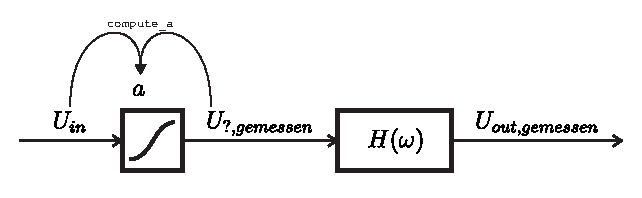
\includegraphics[scale=1.0]{slides/ResultCode/Slide10.eps} 
		}  
	\end{picture} 
	\lstinputlisting[firstline=1,lastline=7]{slides/ResultCode/file.txt} 
}

\ifnum\WertA=2
	\setcounter{onlyAt}{\value{from} + 1}
	\only<\value{onlyAt}>
	{
		\begin{textblock}{20}(65,72)
    		
\includegraphics[scale=0.6 ]{slides/ResultCode/plots/a.JPG} 
		\end{textblock}	
	} 
\fi	
\setcounter{onlyAt}{\value{till}}	


\ifnum\WertA=1 \setcounter{from}{\value{onlyAt}+1} \setcounter{till}{\value{onlyAt}+1} \else \setcounter{from}{\value{onlyAt}+1} \setcounter{till}{\value{onlyAt}+2} \fi	
\only<\value{from} - \value{till}> 
{
	\begin{picture}(100,70)
		\put(15,0)
		{
			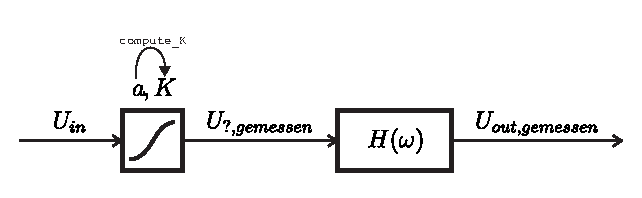
\includegraphics[scale=1.0]{slides/ResultCode/Slide11.eps} 
		}  
	\end{picture} 
	\lstinputlisting[firstline=1,lastline=8]{slides/ResultCode/file.txt} 
}

\ifnum\WertA=2
	\setcounter{onlyAt}{\value{from} + 1}
	\only<\value{onlyAt}>
	{
		\begin{textblock}{20}(80,50)
    		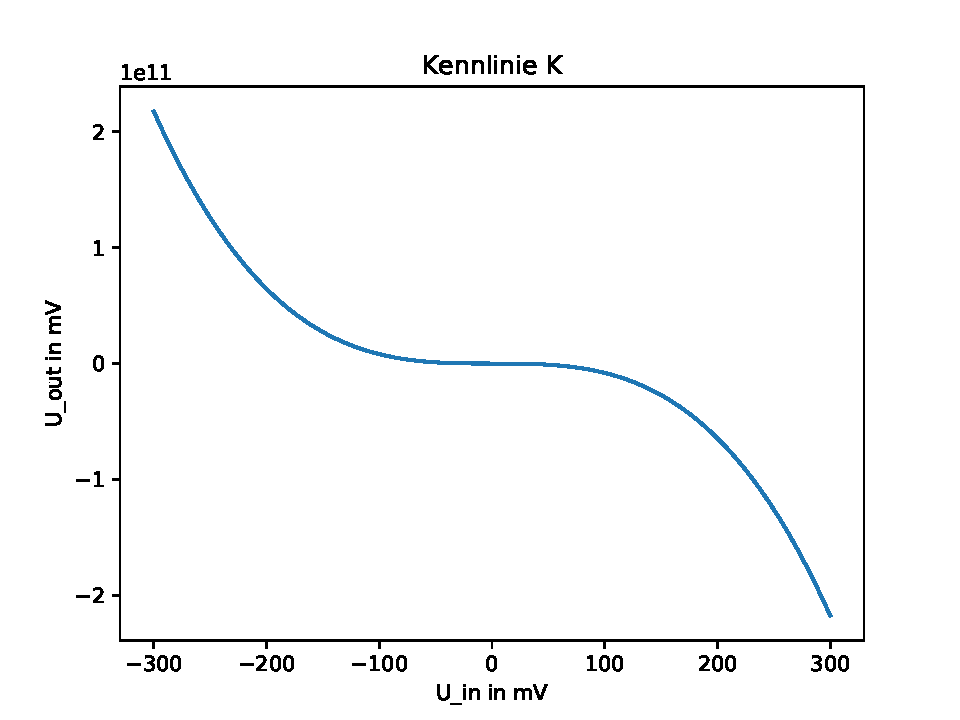
\includegraphics[height=3.5cm, width=4.5cm ]{slides/ResultCode/plots/K.pdf} 
		\end{textblock}	
	} 
\fi	
\setcounter{onlyAt}{\value{till}}	

\setcounter{onlyAt}{\value{onlyAt}+1}
\only<\value{onlyAt}>
{
	\begin{picture}(100,70)
		\put(15,0)
		{
			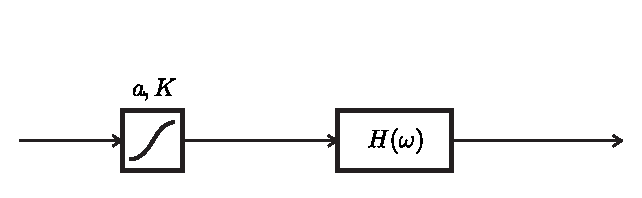
\includegraphics[scale=1.0]{slides/ResultCode/Slide12-0.eps} 
		}  
	\end{picture} 
	\lstinputlisting[firstline=1,lastline=8]{slides/ResultCode/file.txt} 
}
	
\setcounter{onlyAt}{\value{onlyAt}+1}
\only<\value{onlyAt}>
{
	\begin{picture}(100,70)
		\put(15,0)
		{
			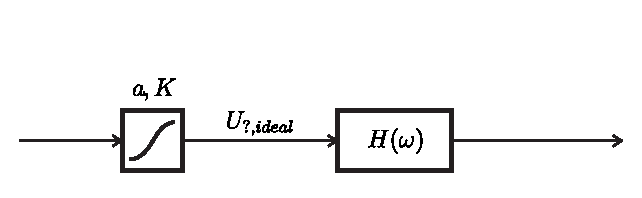
\includegraphics[scale=1.0]{slides/ResultCode/Slide12-01.eps} 
		}  
	\end{picture} 
	\lstinputlisting[firstline=1,lastline=8]{slides/ResultCode/file.txt} 
}
	
\ifnum\WertA=1 \setcounter{from}{\value{onlyAt}+1} \setcounter{till}{\value{onlyAt}+1} \else \setcounter{from}{\value{onlyAt}+1} \setcounter{till}{\value{onlyAt}+2} \fi	
\only<\value{from} - \value{till}> 
{
	\begin{picture}(100,70)
		\put(15,0)
		{
			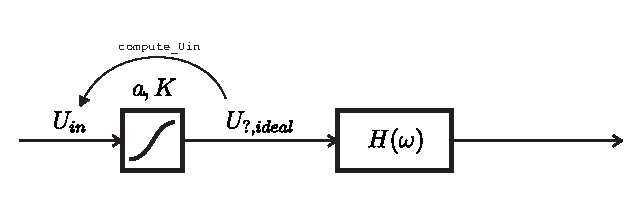
\includegraphics[scale=1.0]{slides/ResultCode/Slide12.eps} 
		}  
	\end{picture} 
	\lstinputlisting[firstline=1,lastline=9]{slides/ResultCode/file.txt} 
}

\ifnum\WertA=2
	\setcounter{onlyAt}{\value{from} + 1}
	\only<\value{onlyAt}>
	{
		\begin{textblock}{20}(80,50)
    		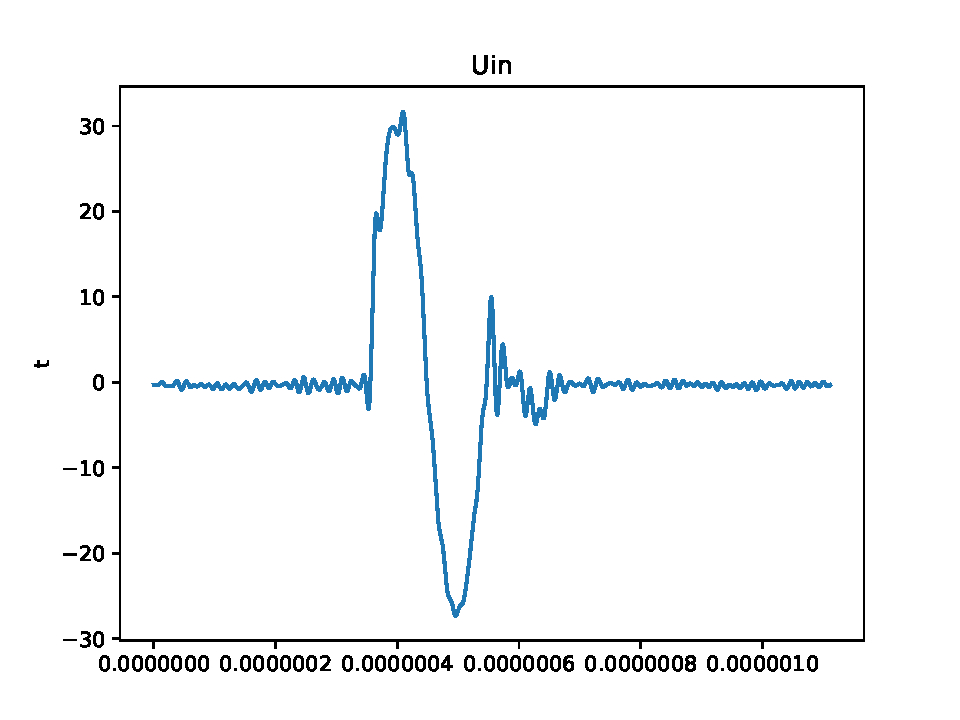
\includegraphics[height=3.5cm, width=4.5cm ]{slides/ResultCode/plots/U_in.pdf} 
		\end{textblock}	
	} 
\fi	
\setcounter{onlyAt}{\value{till}}
	
\setcounter{onlyAt}{\value{onlyAt}+1}
\only<\value{onlyAt}>
{
	\begin{picture}(100,70)
		\put(15,0)
		{
			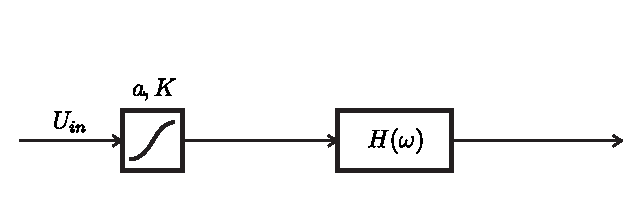
\includegraphics[scale=1.0]{slides/ResultCode/Slide13-0.eps} 
		}  
	\end{picture} 
	\lstinputlisting[firstline=1,lastline=9]{slides/ResultCode/file.txt} 
}



%\setcounter{onlyAt}{\value{onlyAt}+1}
%\only<\value{onlyAt}>
%{
%	\begin{picture}(100,70)
%		\put(15,0)
%		{
%			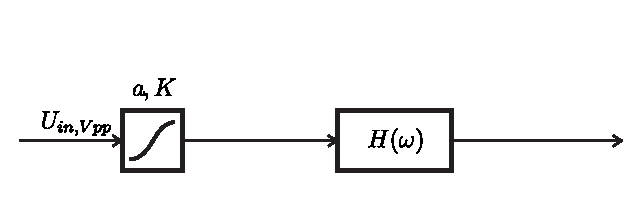
\includegraphics[scale=1.0]{slides/ResultCode/Slide13-01.eps} 
%		}  
%	\end{picture} 
%	\lstinputlisting[firstline=1,lastline=10]{slides/ResultCode/file.txt} 
%}
	
\setcounter{onlyAt}{\value{onlyAt}+1}
\only<\value{onlyAt}>
{
	\begin{picture}(100,70)
		\put(15,0)
		{
			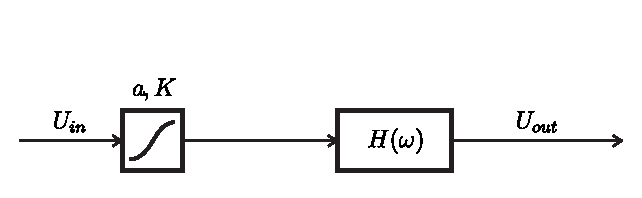
\includegraphics[scale=1.0]{slides/ResultCode/Slide13.eps} 
		}  
	\end{picture} 
	\lstinputlisting[firstline=1,lastline=10]{slides/ResultCode/file.txt} 
}

  
%	\begin{figure}[t]
%	
%%	
%	\end{figure}	
	%}
%\only<2>{ \lstinputlisting[firstline=1,lastline=2]{slides/ResultCode/file.txt} }
%\only<3>{ \lstinputlisting[firstline=1,lastline=3]{slides/ResultCode/file.txt} }
%\only<4>{ \lstinputlisting[firstline=1,lastline=4]{slides/ResultCode/file.txt} }
%\only<5>{ \lstinputlisting[firstline=1,lastline=5]{slides/ResultCode/file.txt} }
%\only<6>{ \lstinputlisting[firstline=1,lastline=6]{slides/ResultCode/file.txt} }
%\only<7>{ \lstinputlisting[firstline=1,lastline=7]{slides/ResultCode/file.txt} }
%\only<8>{ \lstinputlisting[firstline=1,lastline=8]{slides/ResultCode/file.txt} }
%\only<9>{ \lstinputlisting[firstline=1,lastline=9]{slides/ResultCode/file.txt} }
%\only<10>{ \lstinputlisting[firstline=1,lastline=10]{slides/ResultCode/file.txt} }


\end{frame}





%\subsection{Vorgehensweise}
%\begin{frame}
\frametitle{Code: Vorgehensweise}

\only<2->{
\begin{itemize}
	\only<2->{\item Refactoring / Anpassung der Matlab-Funktionen an unser Design}
	\only<3->{\item Portierung der Matlab-Funktionen nach Python}
	\only<4->{\item Überprüfung der portierten Funktionen mithilfe von \textbf{TDD}}
	\only<5->{\item Erweiterung der Blöcken mit \texttt{adjust\_H}   und \texttt{adjust\_a}  }
\end{itemize}
}
 

\end{frame}

%\begin{frame}
\frametitle{\textbf{T}est \textbf{D}riven \textbf{D}evelopment}

\onslide<2->{
\begin{itemize}
	\onslide<2->{\item 27 Unit Tests}
	\onslide<3->{\item 4 System Tests}
\end{itemize}
}
\onslide<4->{Vorteile:
\onslide<5->{
\begin{itemize}
	\onslide<5->{\item Ermöglichen:	
	\begin{itemize}
		\onslide<5->{\item inkrementierende Code-Anpassungen}
		\onslide<6->{\item verteiltes Debuggen ohne den Messaufbau}	
	\end{itemize}		
 	}
	\onslide<7->{\item Zwingen zum modularen Code-Design}
	\onslide<8->{\item Erleichtern das Migrieren der Funktionen aus anderen Sprachen }
\end{itemize}
}
}
 

\onslide<9->{Nachteile:
\onslide<10->{
\begin{itemize}
	\onslide<10->{\item Extra Aufwand: Mehr Code zu debuggen}
\end{itemize}
}
}
 
 

\end{frame}

%\begin{frame}
\frametitle{Das Mock-System}


\onslide<2->{
\begin{itemize}
	\onslide<1->{\item Wird genutzt, wenn mit Geräten kommuniziert wird:	
	\begin{itemize}
		\item \texttt{mock\_system.write\_to\_AWG}
		\item \texttt{mock\_system.read\_from\_DSO}
	\end{itemize}		
 	}
	\onslide<3->{\item Simuliert das Verhalten des Messaufbaus nach dem Hammerstein-Modell}
\end{itemize}
}

\only<4-6>{
		\begin{textblock}{20}(13,37)
    		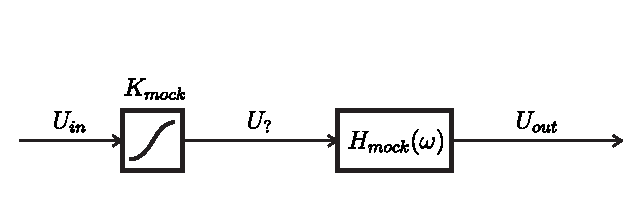
\includegraphics[]{slides/ResultCode/Slide_mock.eps} 
		\end{textblock}		
}
\only<5-6>{
		\begin{textblock}{20}(21,64)
    		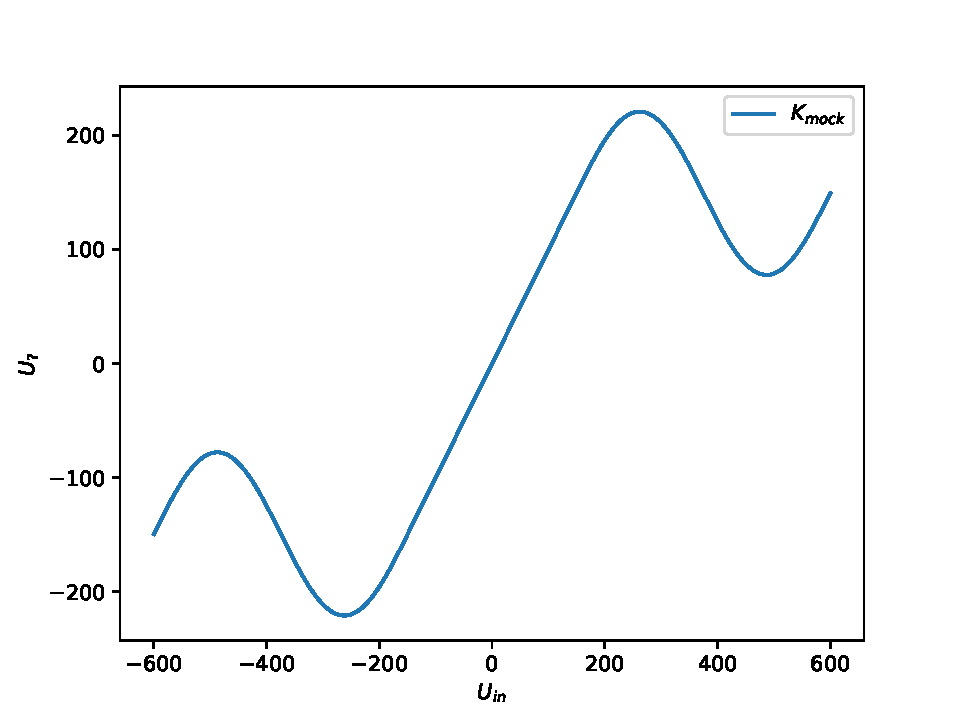
\includegraphics[ width=2.9cm, height=2.4cm ]{slides/ResultCode/plots/K_mock.pdf} 
		\end{textblock}			
}
\only<6>{	
		\begin{textblock}{20}(62,64)
    		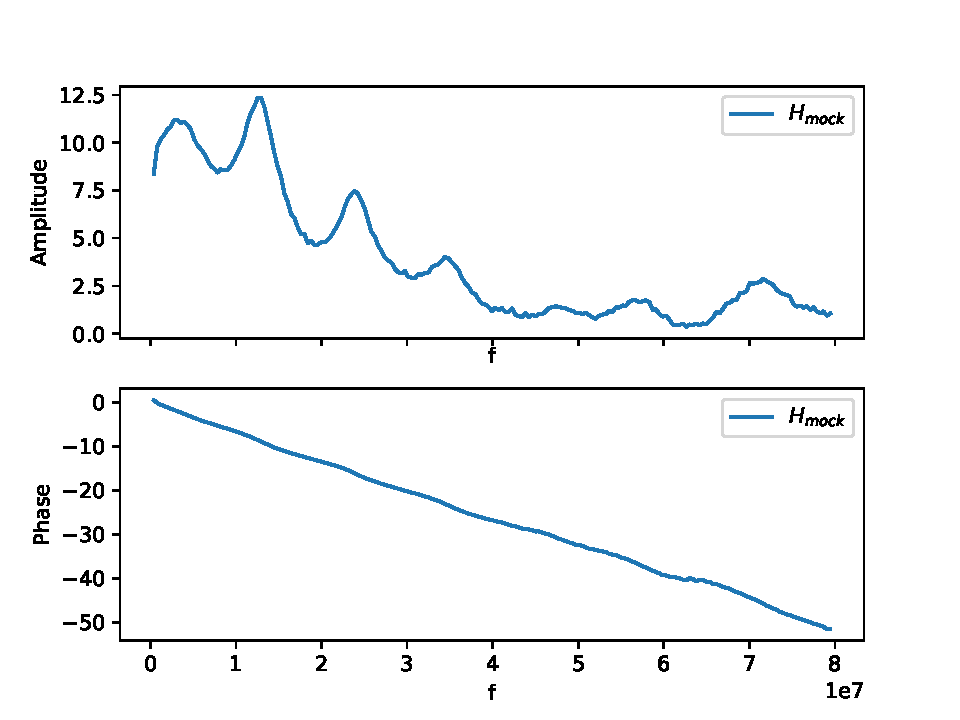
\includegraphics[ width=2.9cm, height=2.4cm]{slides/ResultCode/plots/H_mock.pdf} 
		\end{textblock}	
}



\onslide<7->{Vorteile:
\onslide<8->{
\begin{itemize}
	\onslide<8->{\item Ermöglicht:	
	\begin{itemize}
			\onslide<8->{\item Unit Tests von Bausteinen, in den Gerätekommunikation stattfindet }
			\onslide<9->{\item System Tests }	
			\onslide<10->{\item Testen von Spezialszenarien}
	\end{itemize}		
 	}
	\onslide<11->{\item Hilft das System besser zu verstehen }
\end{itemize}
}
} 

\onslide<12->{Nachteile:
\onslide<12->{
\begin{itemize}
	\onslide<12->{\item Extra Aufwand: mehr Code zu debuggen}
\end{itemize}
}
}
 
 

\end{frame}


\section{Optimierung}
\subsection{Optimierung der Übertragungsfunktion}
%\begin{frame}{Optimierung der Übertragungsfunktion}

\uncover<2->{
Idee: Iterative Anpassung mit
\begin{align*}
			\underline{H}^{i+1} \left( \omega \right) = \underline{H}^{i} \left( \omega \right) \left( 1+ \sigma_H \cdot \left( \frac{\underline{U}_{out,\mathrm{mess}}^{i} \left( \omega \right) }{\underline{U}_{out,\mathrm{ideal}}^{i} \left( \omega \right) } -1 \right) \right) 
		\end{align*}
mit $ \sigma_H $ als Schrittweite.
}
\begin{itemize}
\uncover<3->{
\item Fokus auf Optimierung des Betrags nach ersten Messungen mit Phasenanpassung
}
\end{itemize}

\uncover<4>{
	\begin{picture}(0, -40)
	\put(120, -30){
		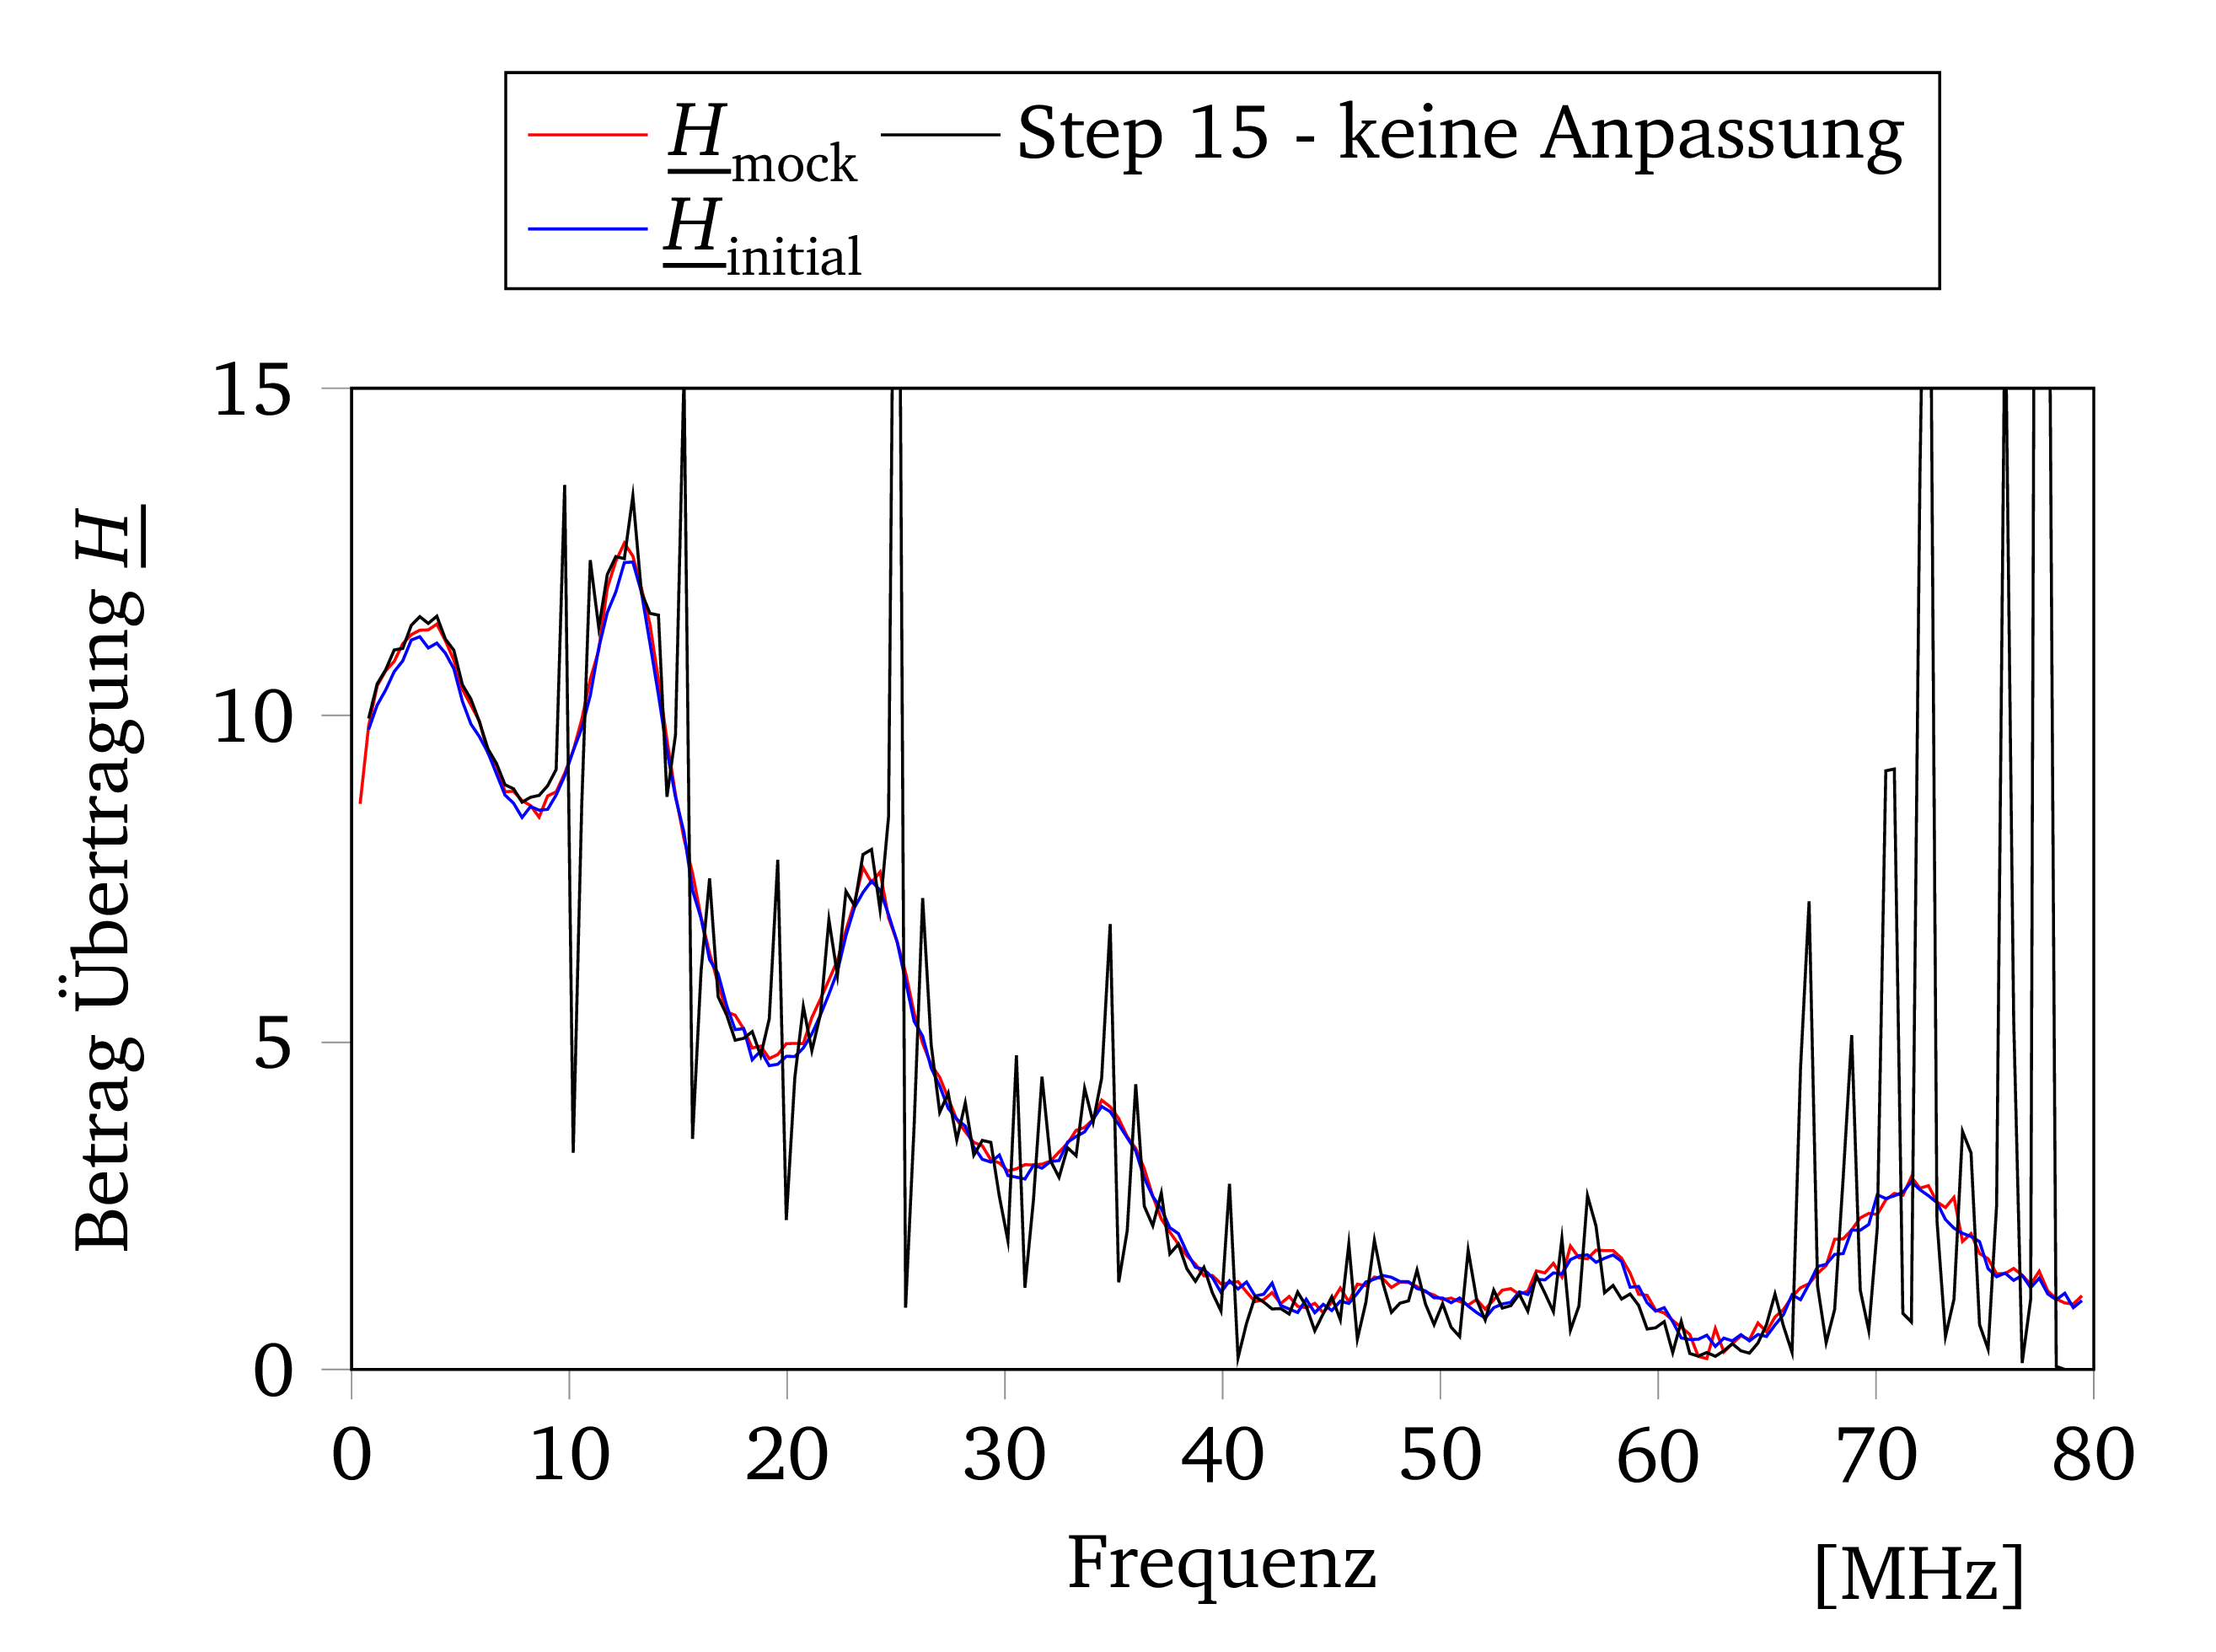
\includegraphics[scale=0.7]{slides/adjust_H/adjust_H_mock.png}	
	}
\end{picture}	
}

%\uncover<2-4, 5->{
%	\begin{picture}(0,70)
%		\put(15,5){
%			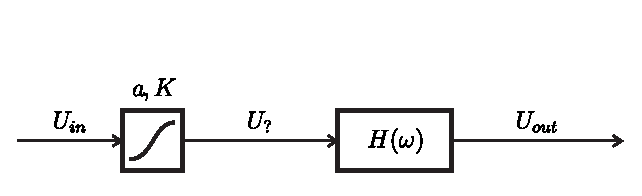
\includegraphics[scale=1.0]{slides/Problemstellung/Slide1.eps} 
%		}
%	\end{picture}
%	}
%

\end{frame}




%\begin{frame}{Optimierung der Übertragungsfunktion}

%\uncover<1-> {
%\begin{align*}
%			\underline{H}^{i+1} \left( \omega \right) = \underline{H}^{i} \left( \omega \right) \left( 1+ \sigma_H \cdot \left( \frac{\underline{U}_{out,\mathrm{mess}}^{i} \left( \omega \right) }{\underline{U}_{out,\mathrm{ideal}}^{i} \left( \omega \right) } -1 \right) \right) 
%		\end{align*}
%}

\uncover<2->{
Fehlerquellen:
}
\begin{itemize}
	\uncover<3->{
		\item Diskretisierungsfehler durch die FFT
	}		
	\uncover<4->{
		\item Interpolationsfehler bei Auswertung des Korrekturterms
	}
	\uncover<5->{
		\item Rauscheinflüsse bei Messungen
	}	
\end{itemize}

\uncover<7->{
Erste Lösungsansätze:
}

\begin{itemize}
	\uncover<8->{
		\item Ignorieren kleiner Beträge in Spektren der Signale
	}
	\uncover<9->{
		\item Ignorieren großer Korrektur-Terme
	}
	\uncover<10->{
		\item \textit{Zero-Padding}
	}
\end{itemize}
\uncover<11->{
$\longrightarrow$ Simulation der komplexen Optimierung am Mock-System
}
\uncover<14->{
\\ \textbf{Ergebnis}: Noch nicht ausgereift
}

%
\uncover<6>{
	\begin{picture}(0, -90)
	\put(170, -38){
		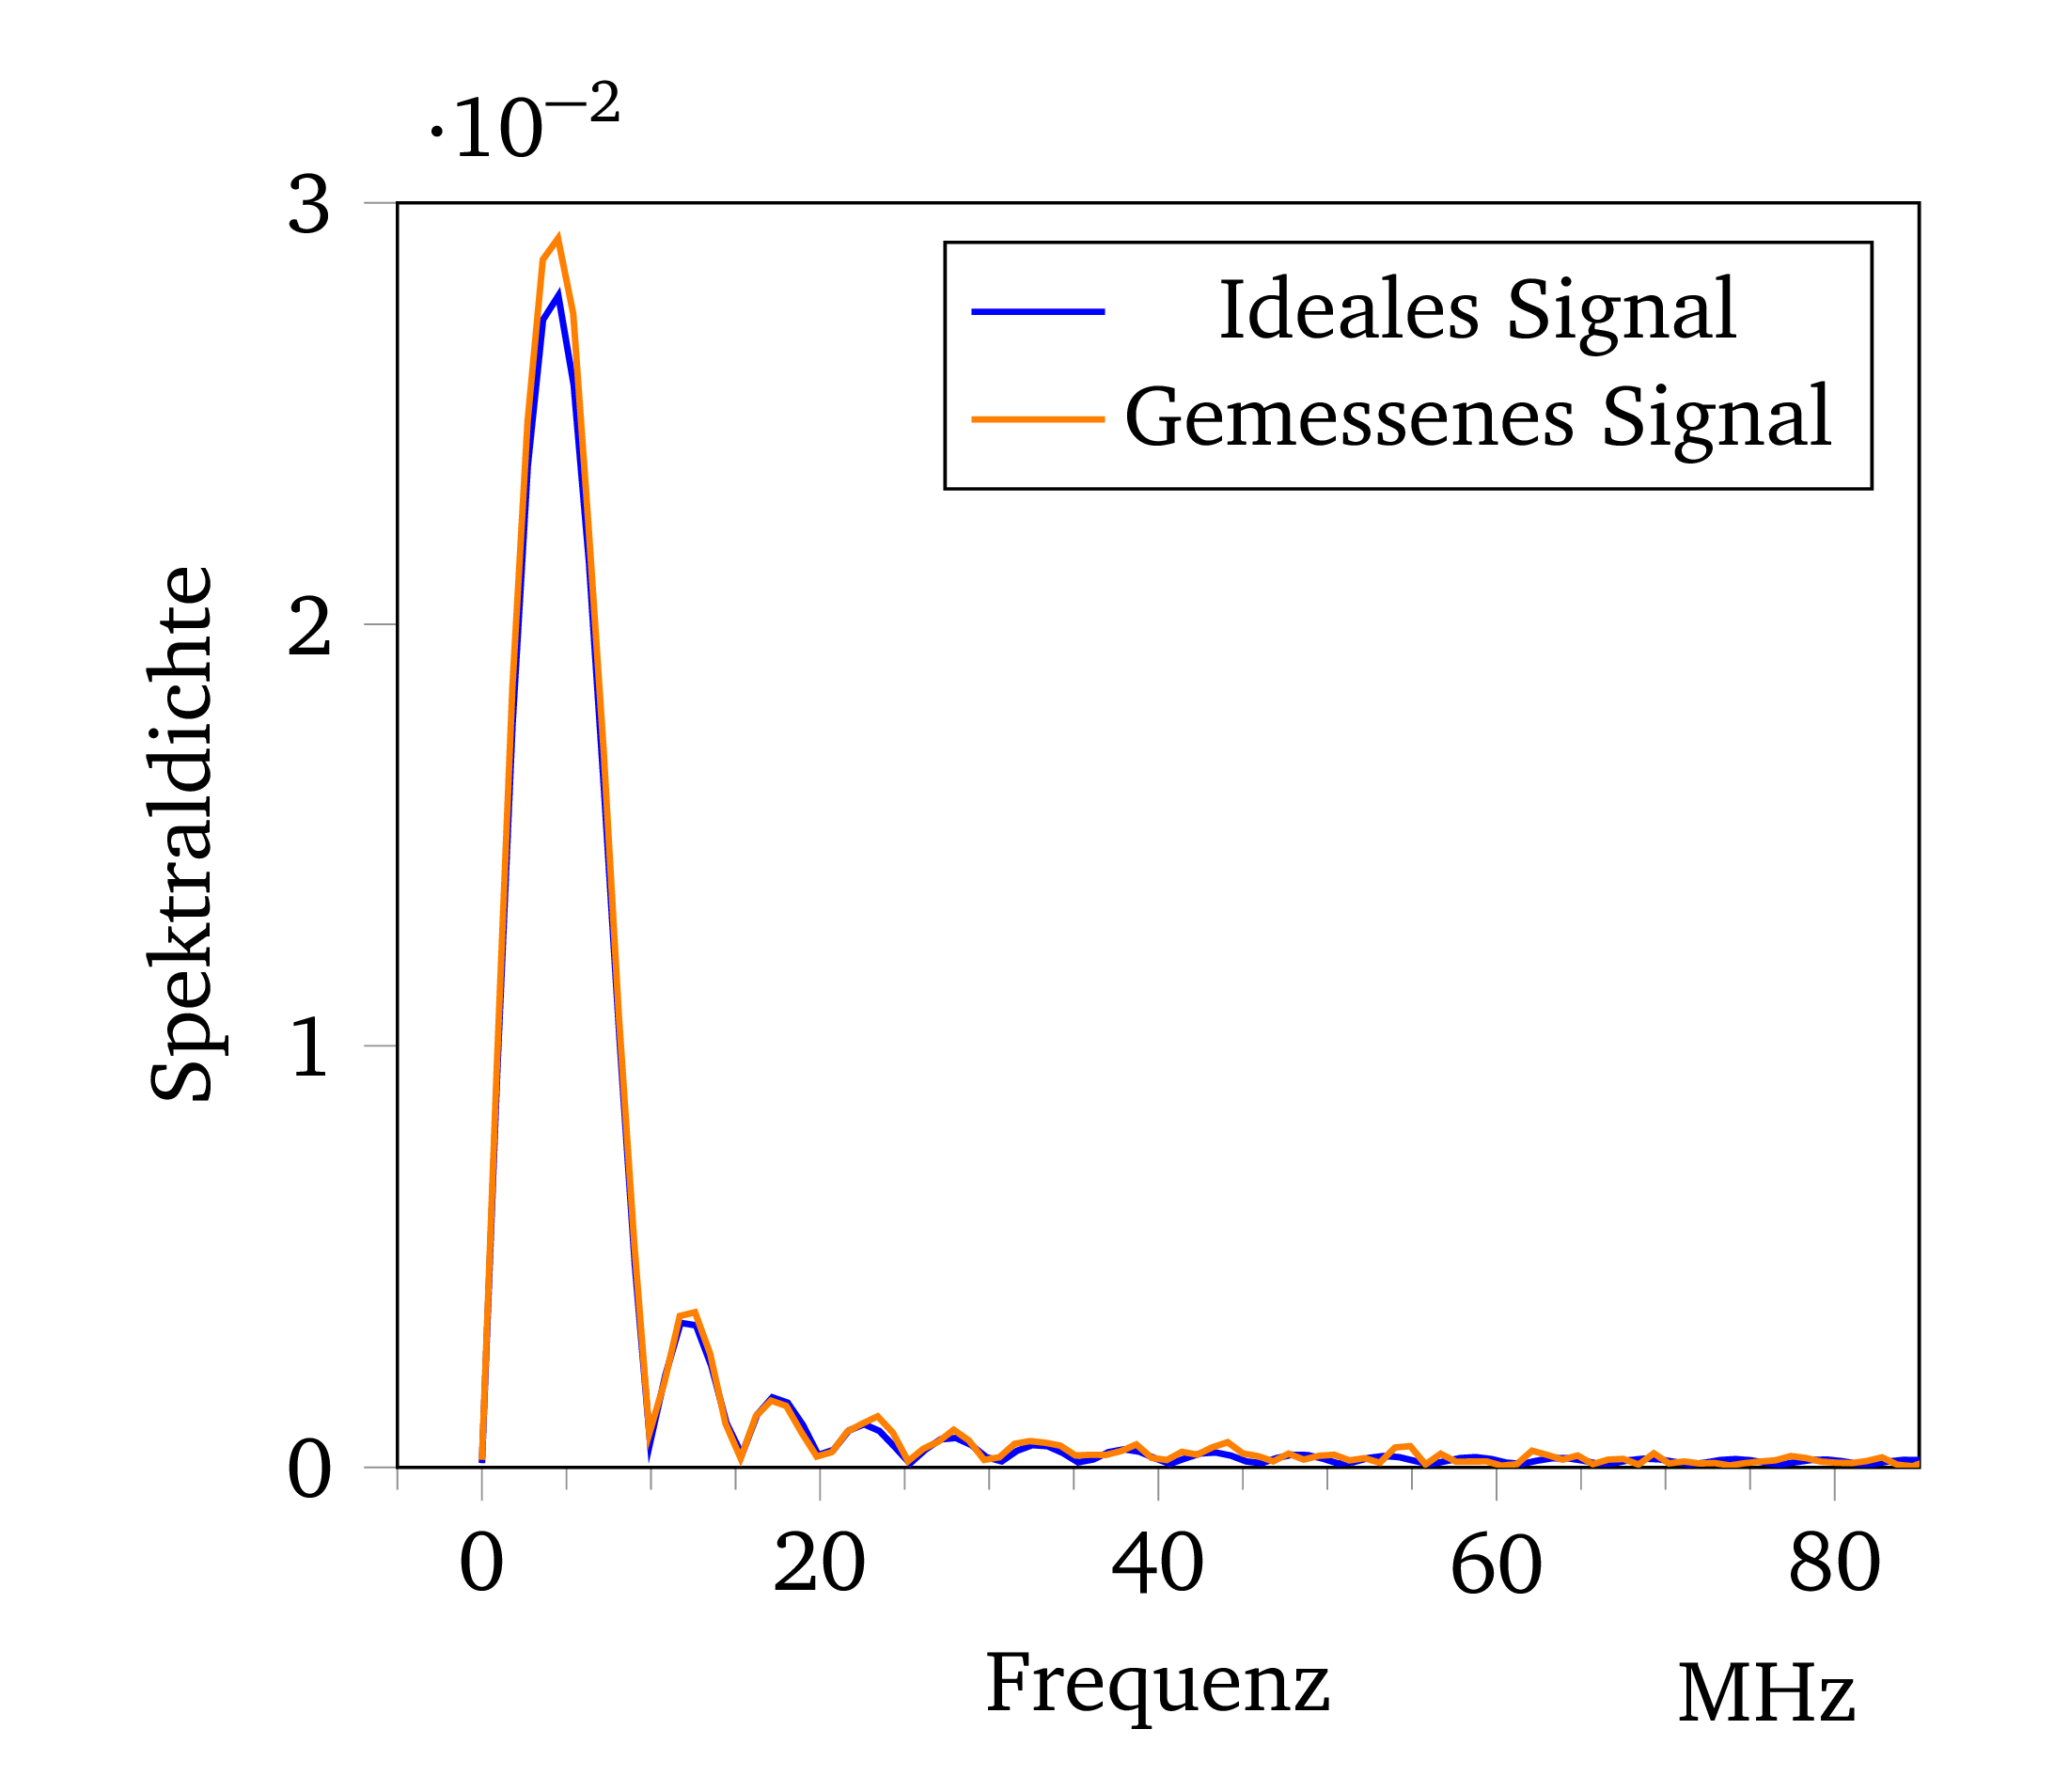
\includegraphics[scale=0.6]{slides/adjust_H/adjust_H_spectre.png}	
	}
\end{picture}	
}


\uncover<12>{
	\begin{picture}(0, -40)
	\put(145, 88){
		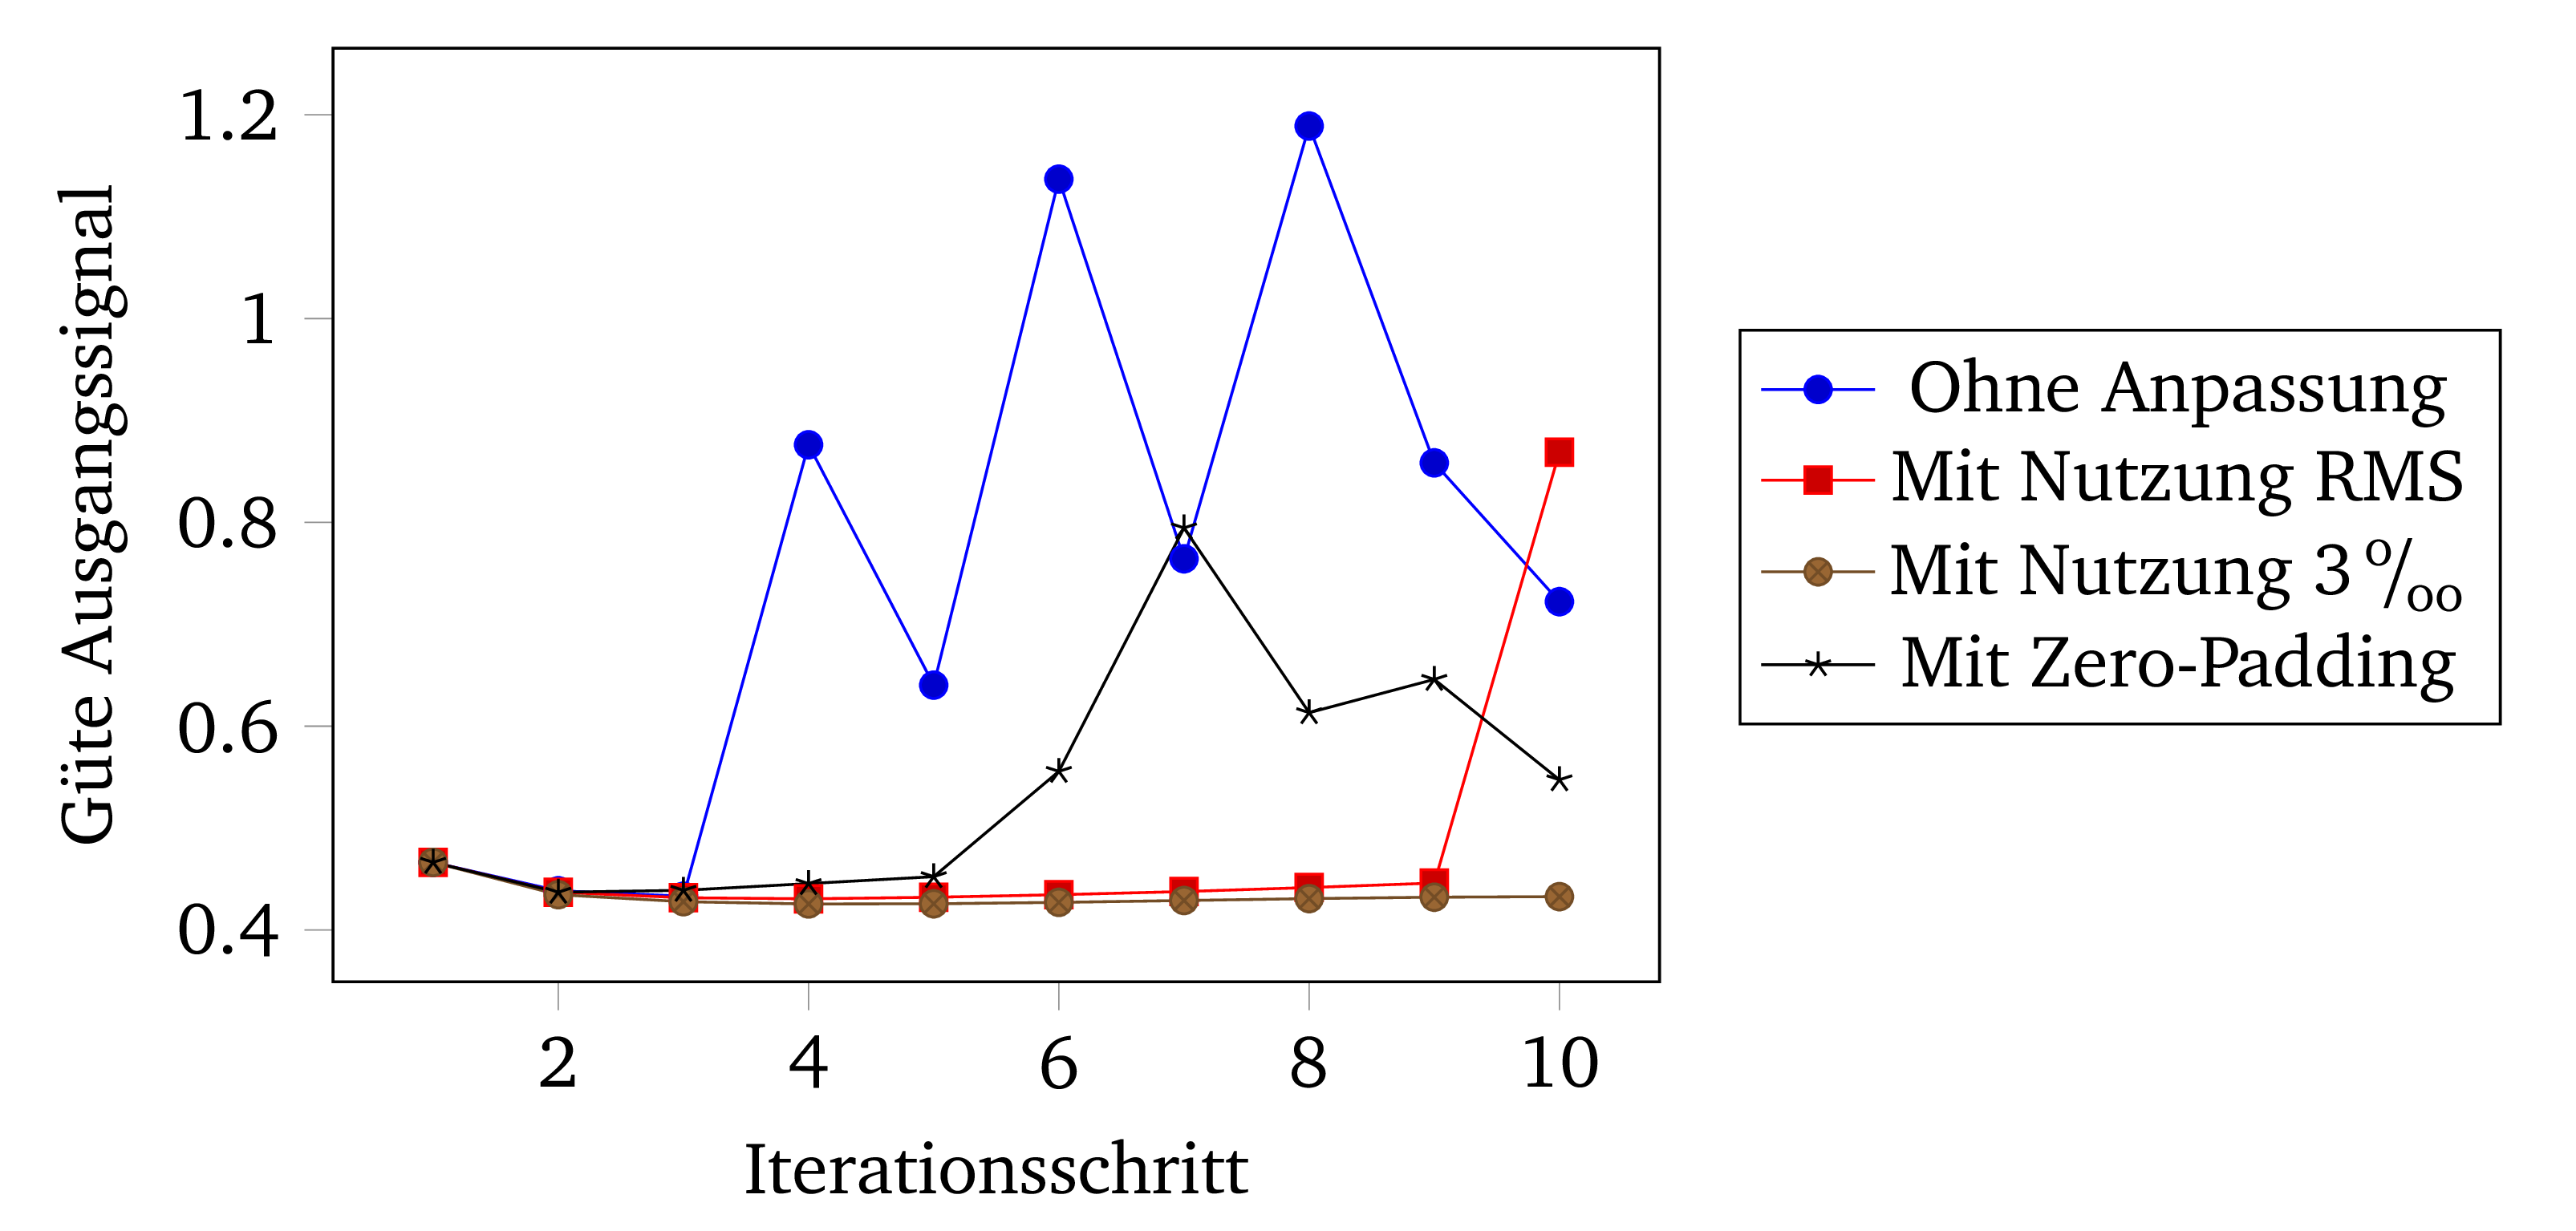
\includegraphics[scale=0.5]{slides/adjust_H/adjust_H_quality.png}	
	}
\end{picture}	
}

%
\uncover<13>{
	\begin{picture}(0, -80)
	\put(177, 70){
		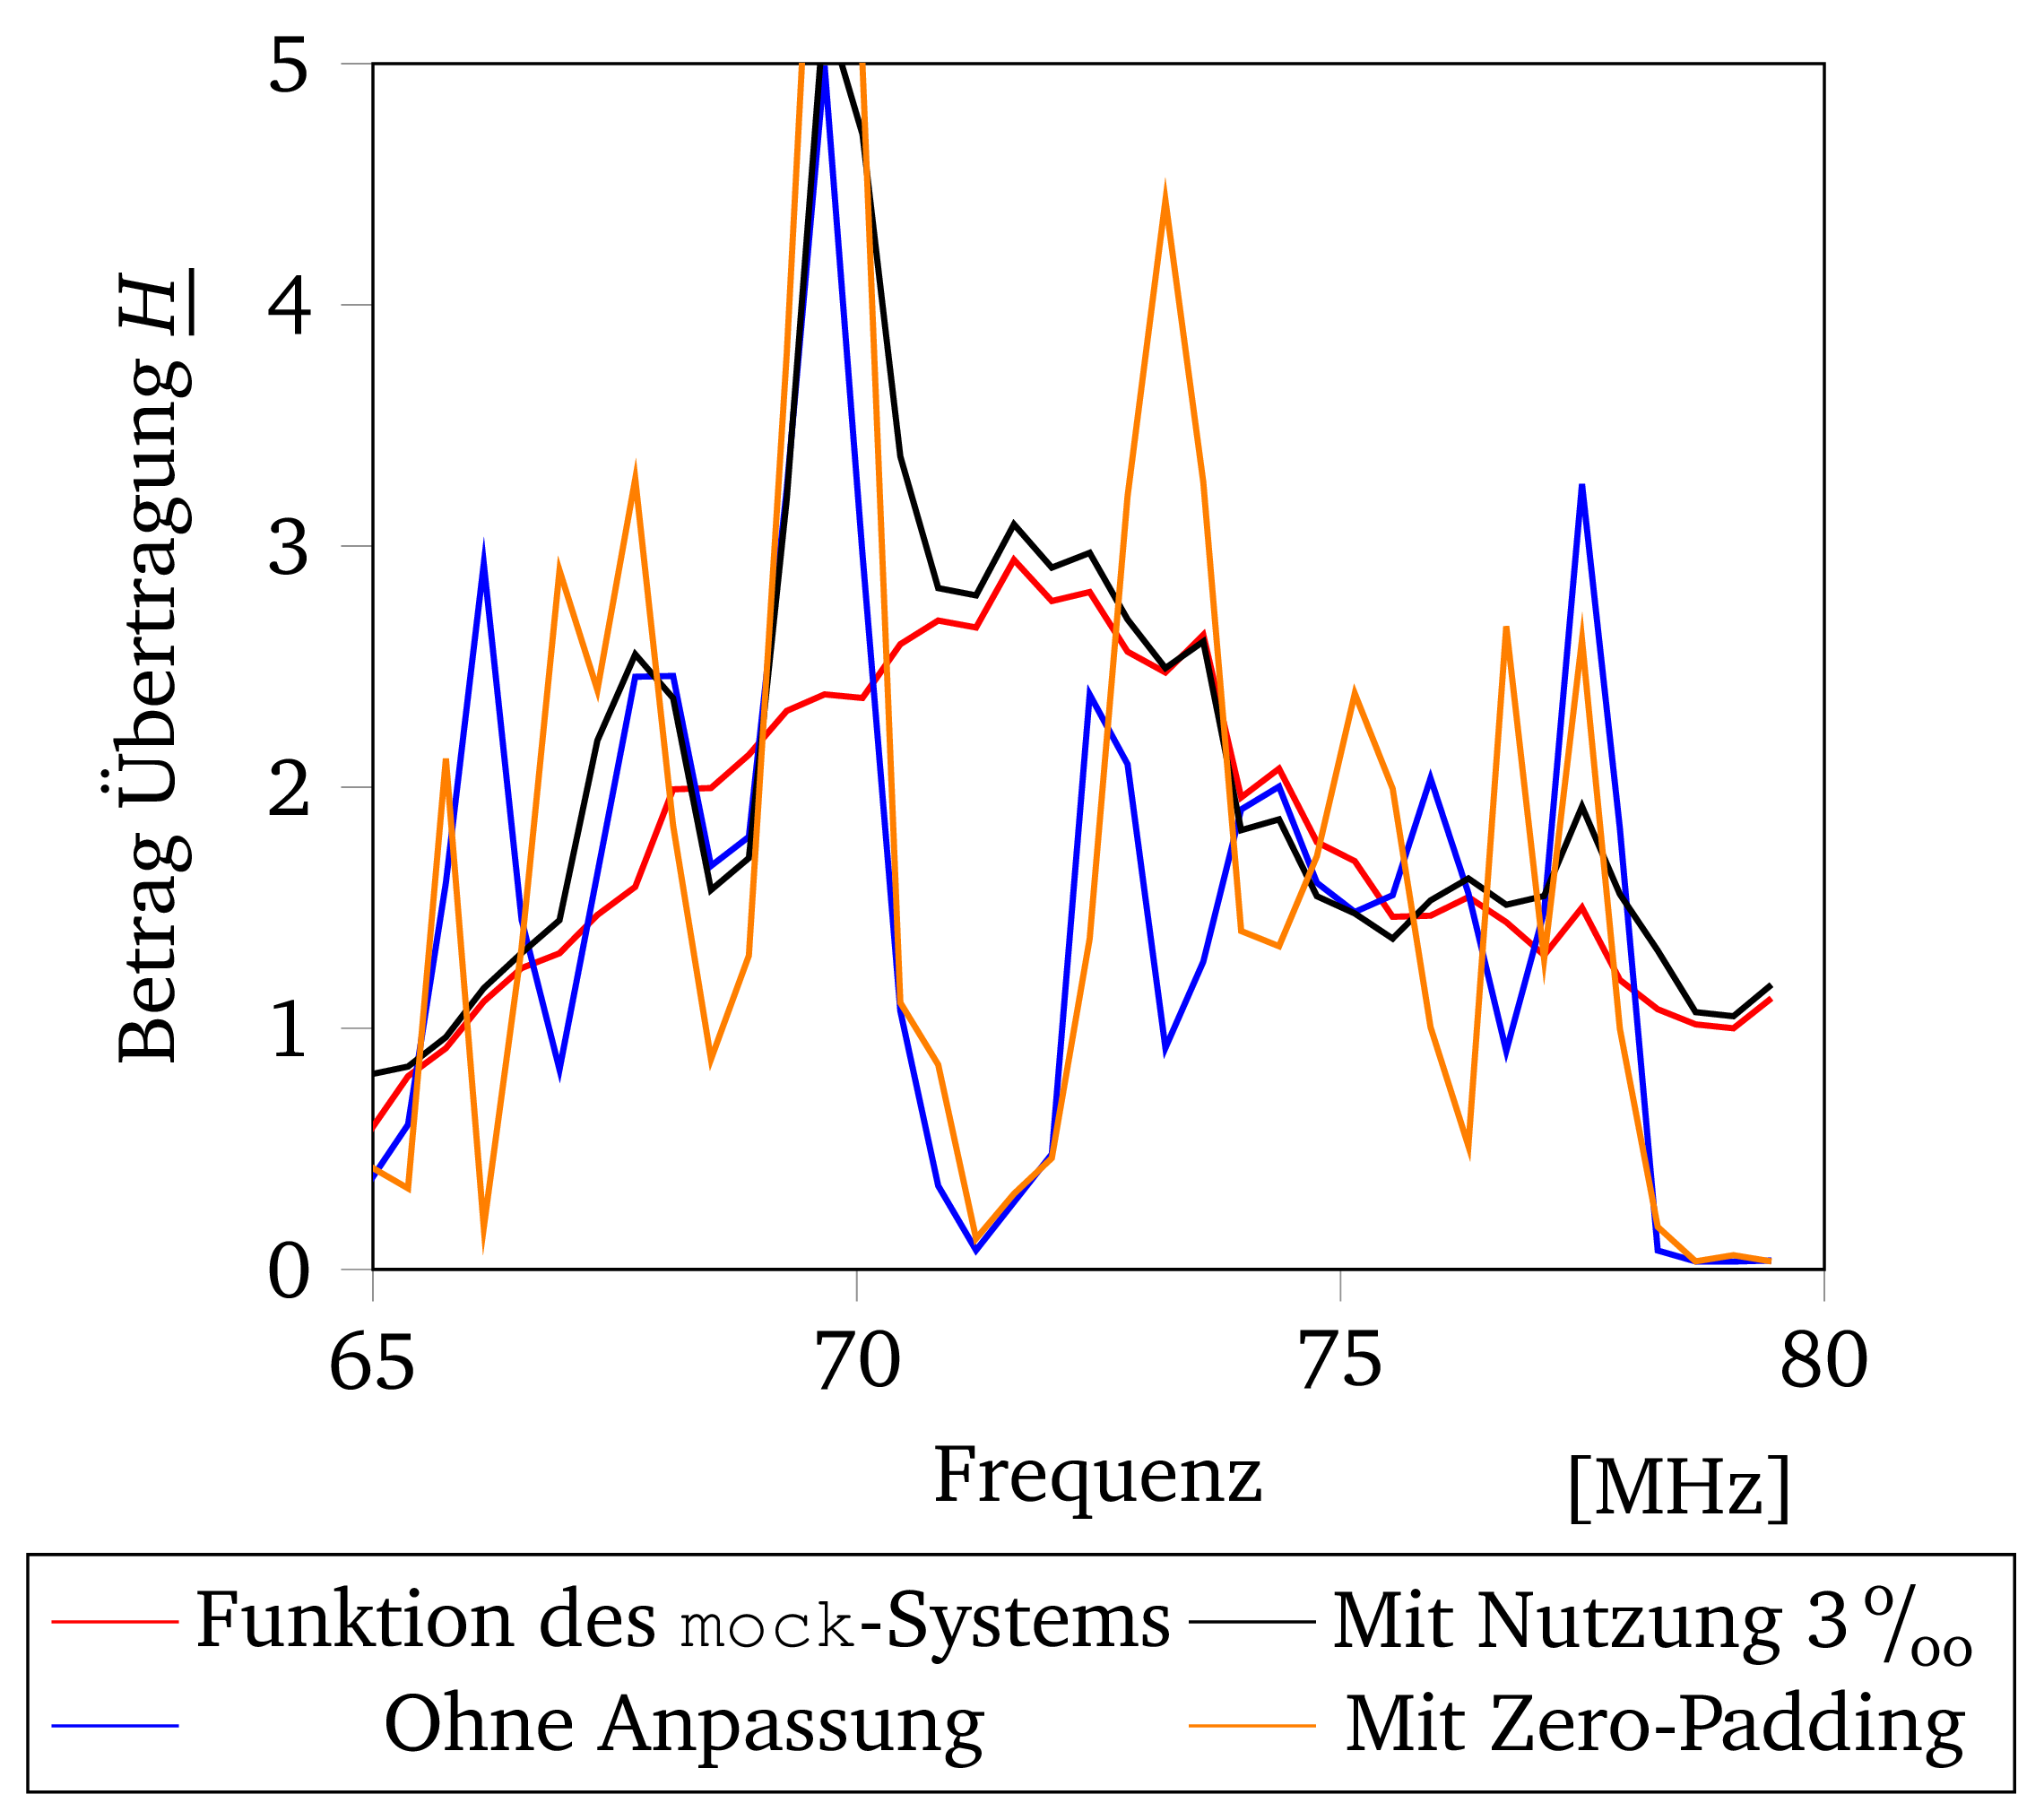
\includegraphics[scale=0.5]{slides/adjust_H/adjust_H_high_frequencies.png}	
	}
\end{picture}	
}


\end{frame}





\subsection{Optimierung der Kennlinie}
\begin{frame}[fragile]
\frametitle{Optimierung von $K$}

\begin{itemize}
  \item Bestimmung von $K$ mit linear vorverzerrten Signal
  \item Anpassung von $K$ für nichtliniear vorverzerrte Signale
\end{itemize}

\begin{align}
	U_{?, \mathrm{meas}} (t) = \sum_{n=1}^N \, \overline{a}_n \left[ U_{in}(t)\right]^n
	\quad
	U_{?, \mathrm{ideal}} (t) = \sum_{n=1}^N \, a_n \left[ U_{in}(t) \right]^n
\end{align}
\begin{itemize}
  \item Oder direkt über die Differenz der Signale
\end{itemize}
\begin{align}
	\Delta U_? (t) = U_{?, \mathrm{meas}} (t) - U_{?, \mathrm{ideal}} (t)
	=
	\sum_{n=1}^N \, \left( \overline{a}_n -  a_n\right) \left[ U_{in}(t) \right]^n
	=
	\sum_{n=1}^N \, \tilde{a}_n \, \left[ U_{in}(t) \right]^n
\end{align}
\end{frame}

\begin{frame}[fragile]
\frametitle{Optimierung von $K$}
\begin{itemize}
	\item Bestimmung der Parameter $\tilde{a}_n$
	\item Vergleichen der Samples ${\Delta U_{?,i} = \Delta U_? (i \cdot \Delta t)}$ mit ${U_{in,i} = U_{in}(i \cdot \Delta t)}$
	\item Lösung des linearen Optimierungsproblems ergibt die Anpassung der alten Parameter
\end{itemize}
\begin{align}
	a_n^{i+1} = a_n^{i} + \sigma_{a}^{i} \tilde{a}_n^{i}
\end{align}
\end{frame}

\begin{frame}
\frametitle{Erster Ansatz}
\begin{itemize}
	\item $K$ im gleichen Spannungsbereich anpassen
	\item Referenz zum Rechnen $U_{out,ideal}$ mit $V_{PP}=\SI{6}{\V}$
	\item Eingangsspannung mit $V_{PP}=\SI{587}{\mV}$
\end{itemize}
\end{frame}

\begin{frame}
\frametitle{Erster Ansatz}
\begin{picture}(10,7)
		\put(0,-160){
			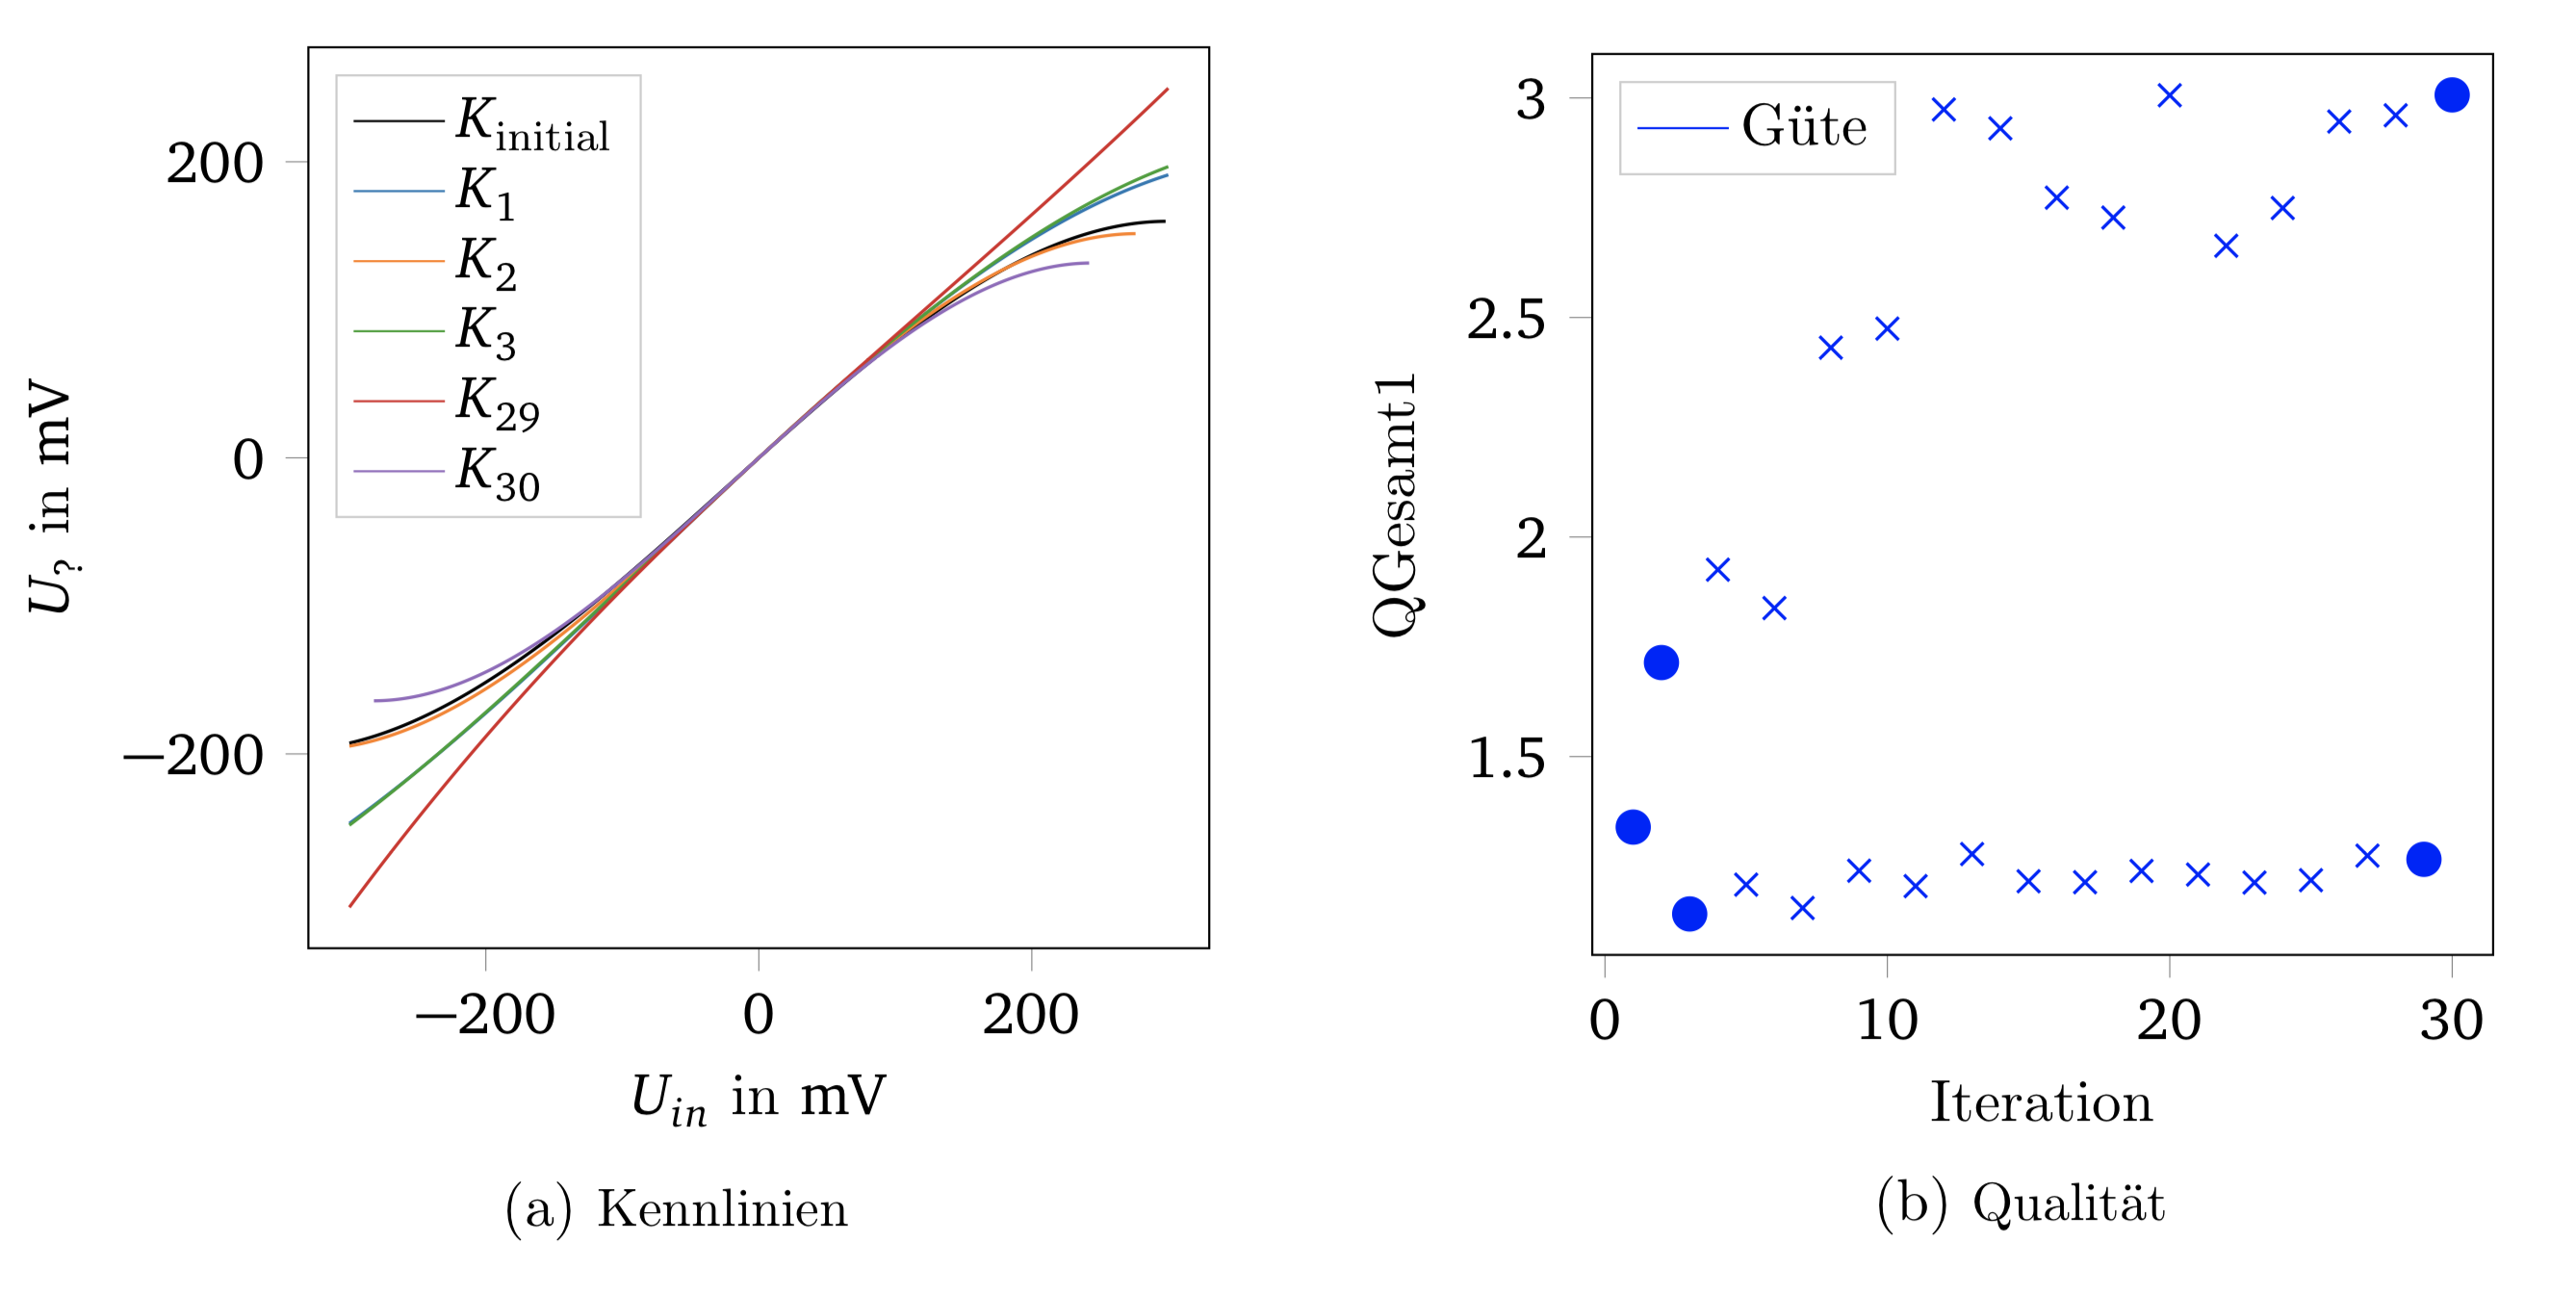
\includegraphics[scale=0.25]{slides/adjust_a/30Iteration.png} 
		}  
	\end{picture}
\end{frame}
\begin{frame}
\frametitle{Grenzen der Kennlinie}
\begin{picture}(10,7)
		\put(0,-160){
			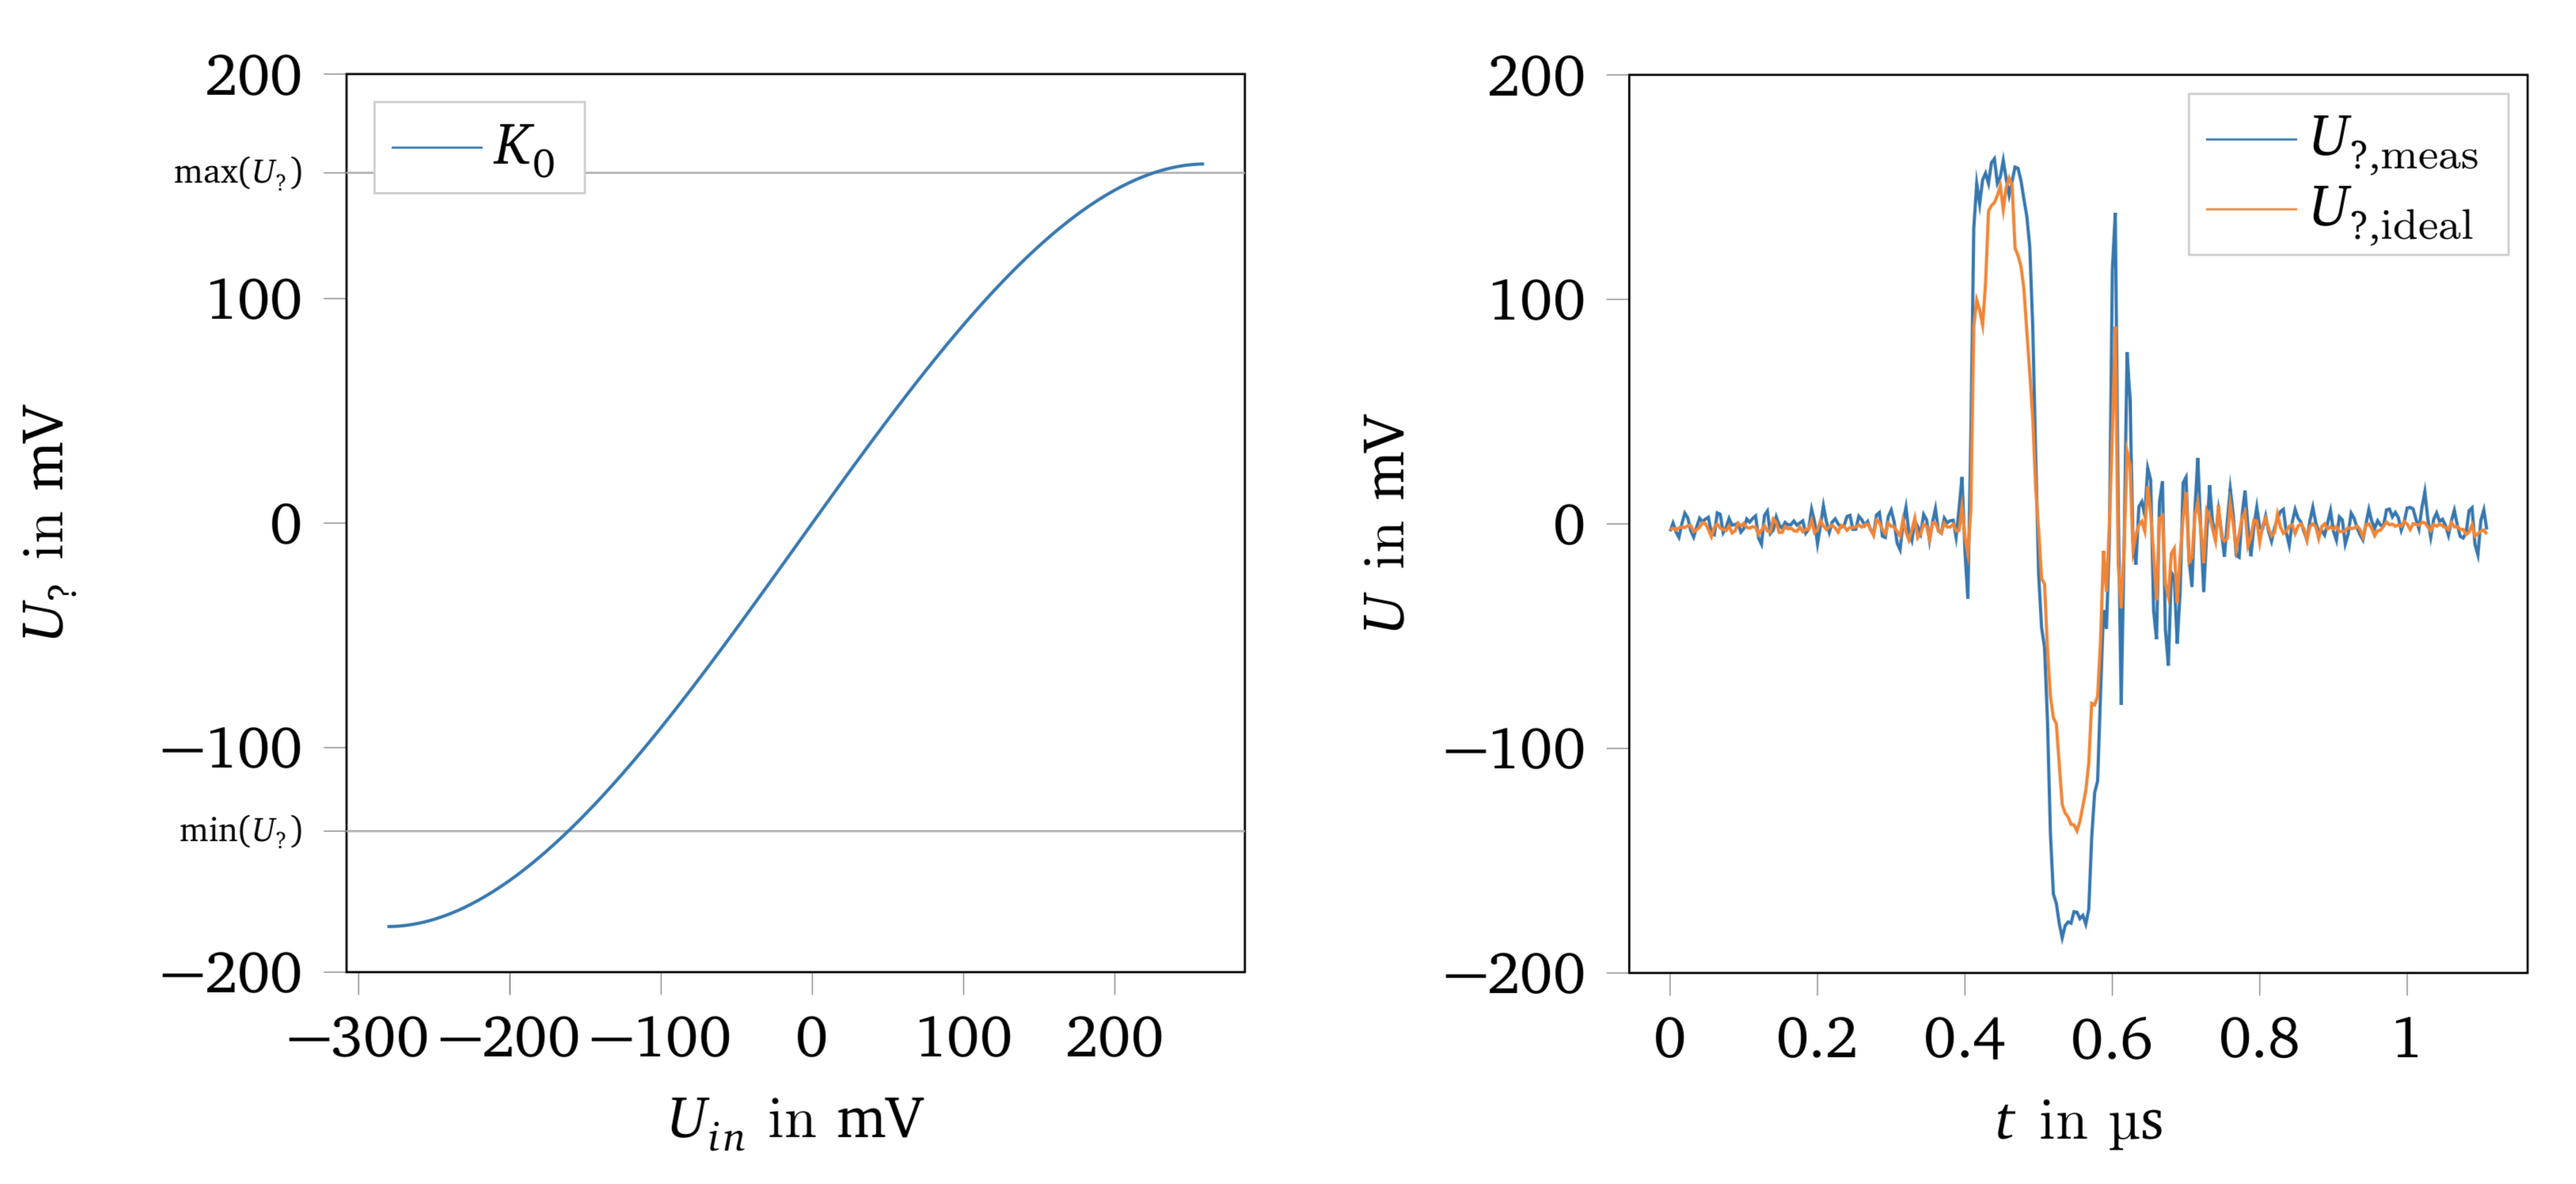
\includegraphics[scale=0.2]{slides/adjust_a/Grenzen_K.png} 
		}  
	\end{picture}
\end{frame}
\begin{frame}
\frametitle{Grenzen der Kennlinie}
\begin{picture}(10,7)
		\put(-5,-160){
			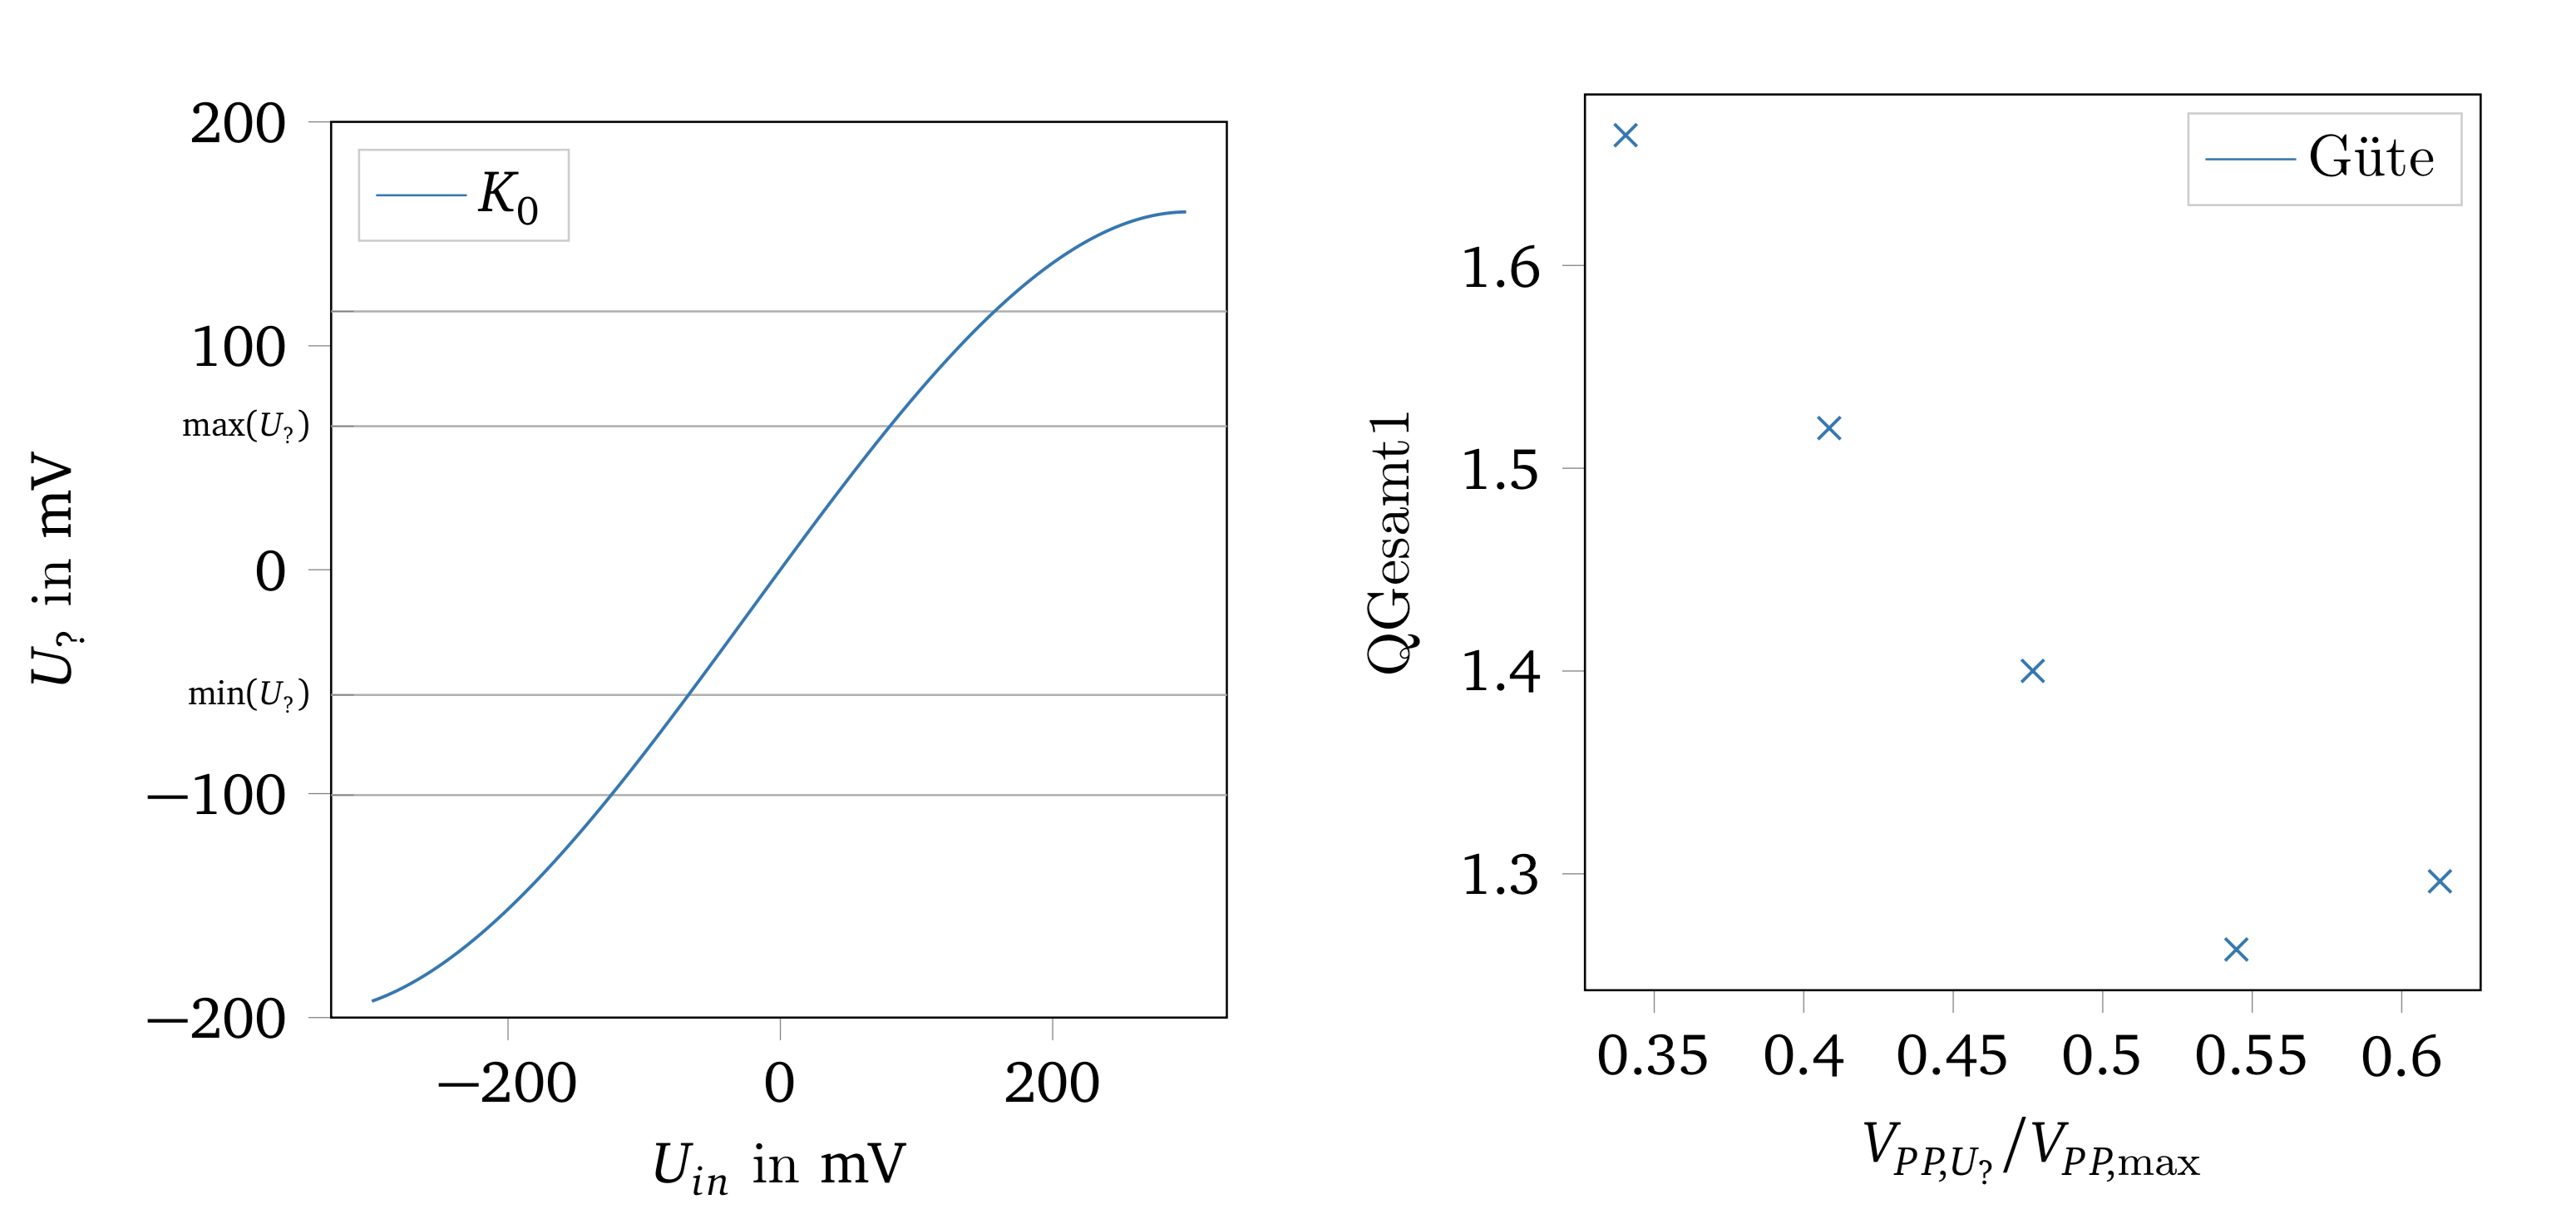
\includegraphics[scale=0.22]{slides/adjust_a/Grenzen_eval.png} 
		}  
	\end{picture}
\end{frame}
\begin{frame}
\frametitle{Zweiter Ansatz}
\begin{itemize}
	\item $K$ in einem kleineren Spannungsbereich anpassen
	\item Referenz zum Rechnen $U_{out,ideal}$ mit $V_{PP}=\SI{3}{\V}$
	\item Eingangsspannung mit $V_{PP}=\SI{290}{\mV}$
	\item Ausgangsspannung gemessen über Gapspannungsteiler $V_{PP}=\SI{2,7}{\V}$
\end{itemize}
\end{frame}

\begin{frame}
\frametitle{Zweiter Ansatz}
\begin{picture}(10,7)
		\put(-5,-160){
			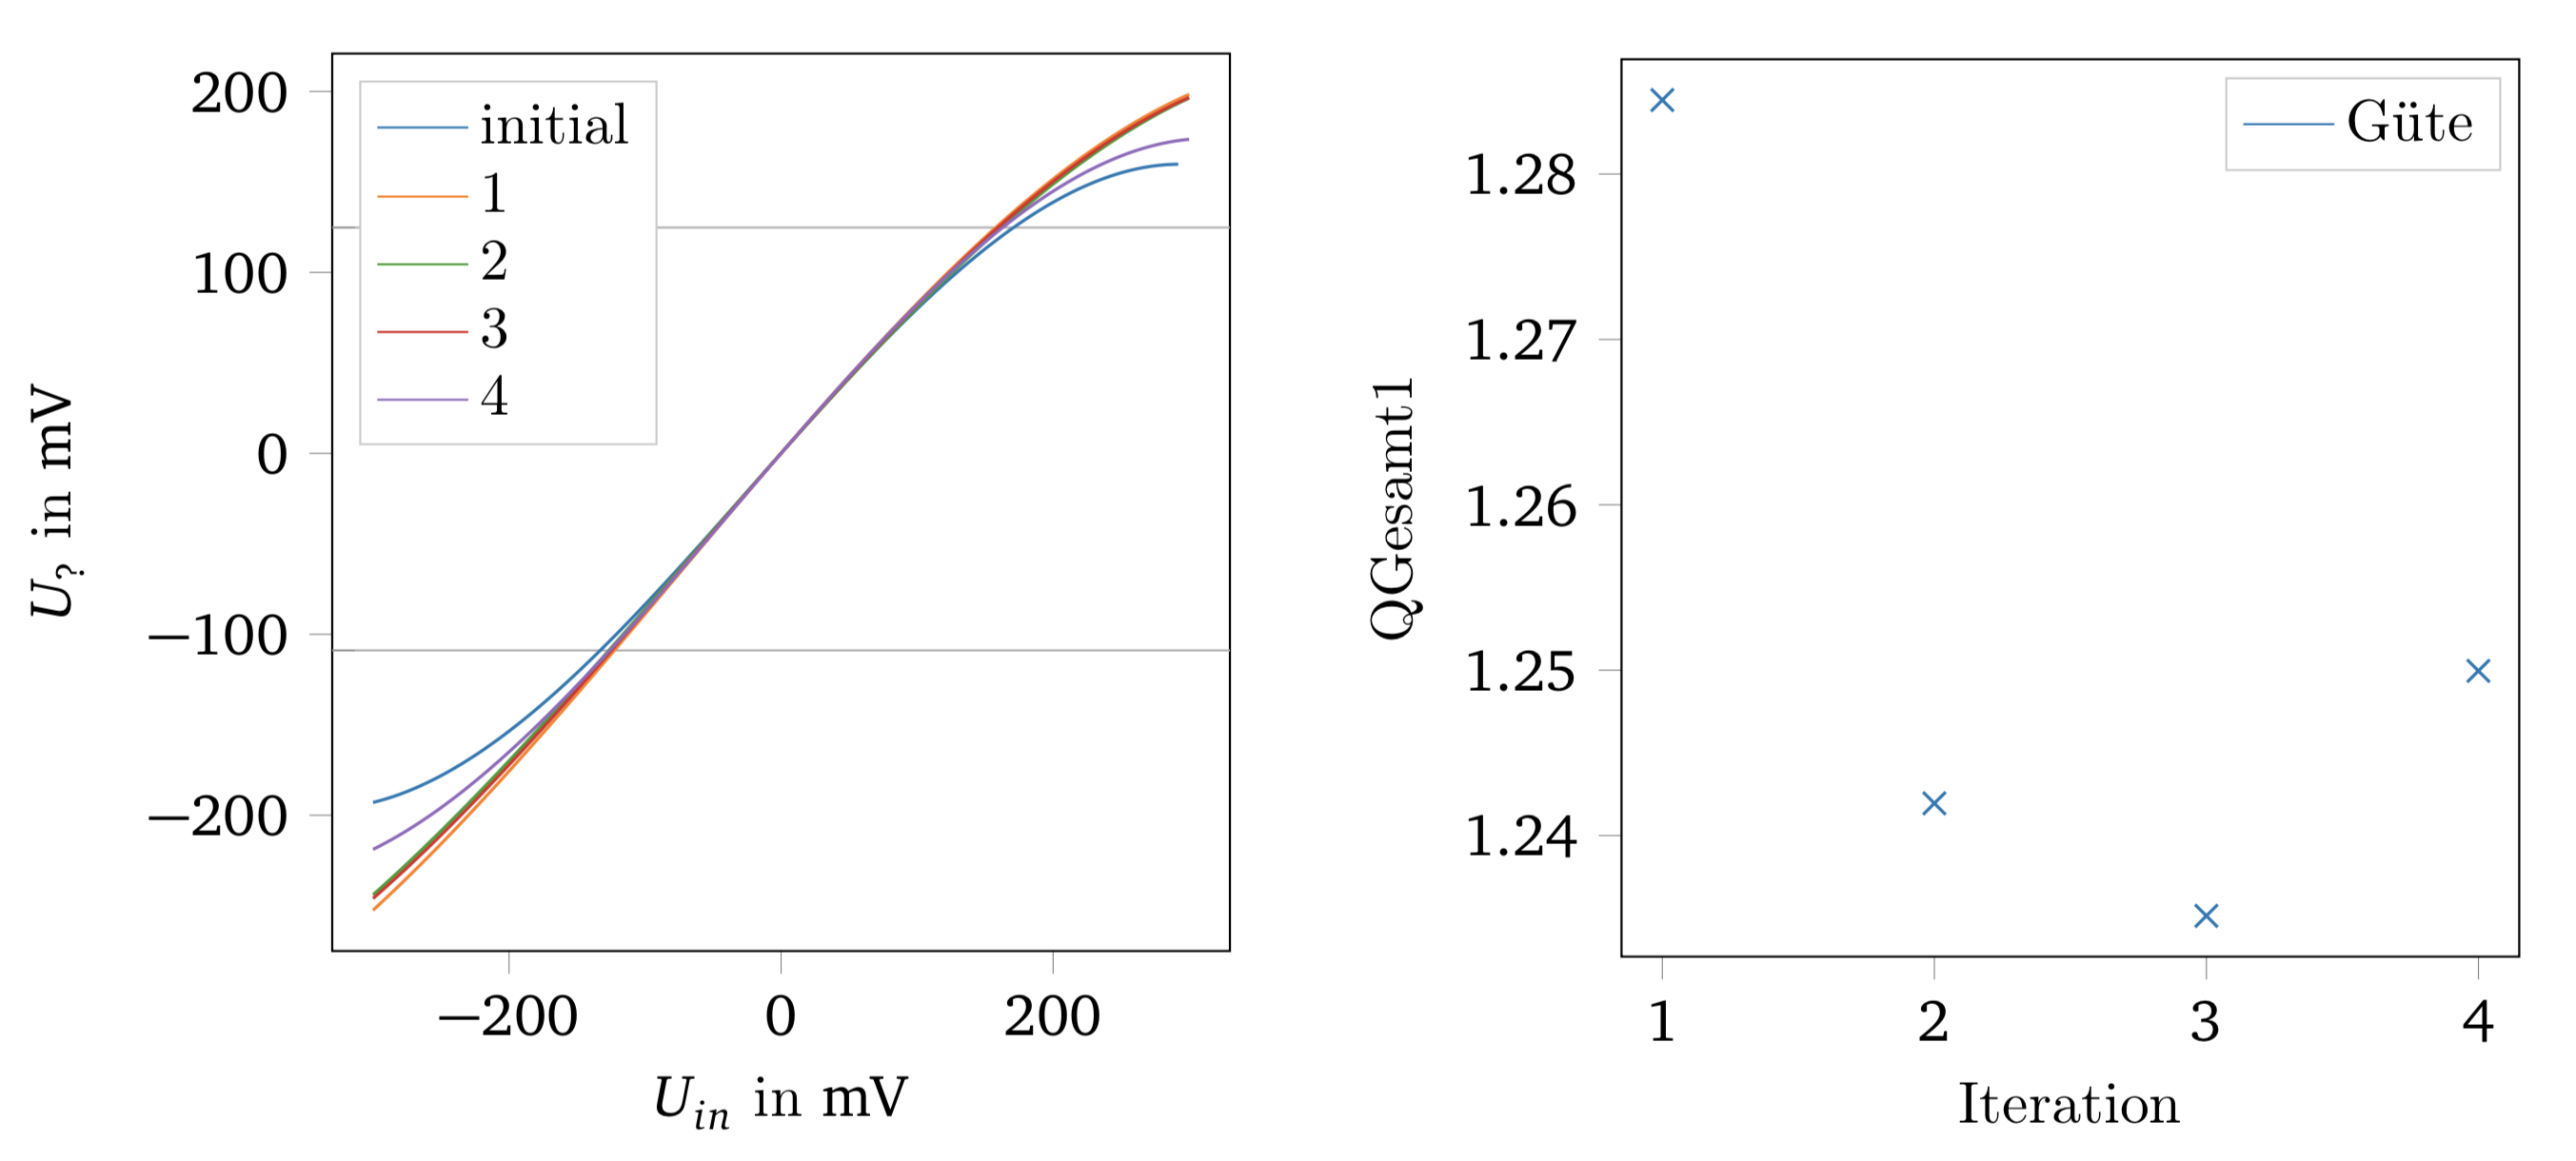
\includegraphics[scale=0.25]{slides/adjust_a/Zweiter_Versuch.png} 
		}  
	\end{picture}
\end{frame}


%\section{Ausblick}
%\documentclass[../Report.tex]{subfiles}


\begin{document}


\chapter{Ausblick}
\label{chap:ausb}
---- In diesem Kapitel wird auf offene Fragen / neue Probleme / Anstöße für weitere Arbeiten eingegangen. Dabei sollte es um eher inhaltliche Aspekte gehen (u. U. wenig to dos für Code-Design) gegebenenfalls darf hier bei vielem auf die Erfahrungen aus den vorigen Kapiteln verwiesen werden und damit einen Übersichts-Charakter haben (erleichtert nachfolgenden Projekten die Arbeit) --- 

\section{Impressionen zum Code}
\label{sec:ausb.code}
In Bezug auf das Design des Codes verbleiben eine Reihe Anregungen und Gedanken, die nicht realisiert wurden, je nach Ausführung aber interessant zu bedenken sein könnten.

\begin{itemize}
	\item	Die Geräte AWG und DSO als Klassen einzubinden könnte den Vorteil bieten, alle SCPI Commands an einer Stelle zu bündeln und den Zugriff darauf allgemeingültig zu halten.
	
	\item	Eine Einbindung des momentanen Programms in die RF-Tools des GSI-Standards könnte in zwei Teilen erfolgen. Die bestehende Funktionalität zur Berechnung von $K$ und $\Hcompl$ kann unabhängig der Optimierungsalgorithmen genutzt werden. Dabei ist insbesondere zu prüfen, ob oder wie die Aspekte im \nameref{chap:code} beibehalten werden. 
	
	\item 	Die momentane Version ist in erster Linie über eine Python-IDE ausführbar. Die Ausführung über die Kommandozeile wurde nicht fokussiert.
	\item Für die Erstellung eines idealen Barrier-Bucket Ausgangssignals wird momentan noch eine selbst implementierte Methode verwendet. Dafür kann auch das vorhandene RF-Tool verwendet werden.
	
\end{itemize}





\section{Ausblick: Optimierung}
\label{sec:ausb.opti}

- (offene Punkte K-Optimierung?)


Auf den Ergebnissen aus \nameref{chap:opt} aufbauend, verbleiben eine Reihe von offenen Fragestellungen:

\begin{enumerate}
	\item 	Wie wirkt sich die Optimierung von $K$ aufgrund ihrer Nichtlinearität auf die Übertragungsfunktion $\Hcompl$ aus und muss dies in der Optimierung berücksichtigt werden, etwa in der Reihenfolge der Iterationsschritte?
	
	\item	Wie wird mit der Tatsache umgegangen, dass im Frequenzbereich unabhängig der Qualität der Messung nur etwa halb so viele Daten für die Anpassung zur Verfügung stehen, wie in $\Hcompl$ selbst vorliegen?
	
	\item 	Ist die getrennte Interpolation von Betrag und Phase der Signalspektren auf die Frequenzen der Übertragungsfunktion in der Optimierung von $\Hcompl$ die beste Lösung? 
	
	\item	In welcher Reihenfolge wird die Iteration durchgeführt? Wird zuerst $\Hcompl$ in mehreren Durchgängen angepasst und danach $K$? Oder im Wechsel je eine Iteration?
	
	\item 	Wie wird die Auswahl der Schrittweiten $\sigma_H$ und $\sigma_a$ vorgenommen? Werden diese pauschal einmal festgesetzt zu Beginn des Algorithmus oder ist eine dynamische Anpassung, etwa durch die Qualität des letzten gemessenen Signals oder in Abhängigkeit des Iterationsschritts vorzuziehen? 
	
	\item 	Wie lässt sich der Einfluss von zufälligem Rauschen auf die Optimierung reduzieren? Insbesondere die Auflösung im höherfrequenten Betragsspektrum ist hier problematisch. Und im Falle des Ignorieren von Korrekturen an als fehlerhaft befundenen Frequenzen: Auf welchen Wert wird der Korrekturterm bei diesen Frequenzen gesetzt?
	
	\item	Wie lassen sich die im idealen Spektrum des Einzelsinus enthaltenen Nulldurchgänge in der Optimierung von $\Hcompl$ berücksichtigen, um interpolationsbedingt große Fehlerterme zu vermeiden? Ist das einfache Ignorieren dieser Frequenzen für die Anpassung eine Möglichkeit? Und in welchem kleinen Frequenzbereich um einen Nulldurchgang müssten dann die Werte ignoriert werden?
	
	\item 	Wie - insofern überhaupt - ist eine Optimierung der Phase von $\Hcompl$ zu gestalten?
	
	\item	Nach welchem Qualitätsmerkmal wird das Signal bewertet und wie wirkt sich dies auf den Algorithmus aus?
	
	\item	Gibt es eine sinnvolle Abbruchbedingung, mit der die Iteration versehen werden sollte? Etwa, dass sich die Qualität im Vergleich zu den vorherigen Iterationen nicht mehr mit ähnlicher Rate verbessert hat? Der Trade-Off liegt zwischen Laufzeit und Signal-Qualität.
	
	\item	Wie bestimmt man die Grenzen, in denen $K$ genutzt werden kann? Wie kann man garantieren, dass $K$ in den Bereichen, aus denen die Daten zur Berechnung von $a_n$ benutzten werden, bijektiv ist?
	
	\item	Gibt es eine Möglichkeit die Grenzen von $K$ bei der Optimierung zu erweitern? Ein möglicher Indikator: Kann man die Rückgabe von \lstinline{numpy.linalg.lstsq(LGS)} aus der Berechnung von $a_n$ nutzen, um eine Aussage über die Abweichung der Werte zu treffen?
\end{enumerate}





\section{--- Gerätekomm---}
\label{sec:ausb.geraete}
--- in dieser Section werden weitere Punkte der Geräte-Komm aufgegriffen, etwa - die (geringe) Auflösung des AWG im Kontext der Optimierung (ggf. in \ref{sec:ausb.opti} besser?) , die Einbindung des neuen Oszis oder die Idee der Klassen-Implementierung 
%TODO: prüfe Redundanz mit Abschnitt Gerätekommunikation! nur eine Einbindung, wo ist sie sinnvoller? 

%TODO: Überlegung ausführen, ob RF-Tools einbinden hier sinnvoller ist als in "Offenen Fragen" im Abschnitt Code-Design?






\end{document}
%\begin{frame}
\frametitle{Empfehlungen zum Code-Design}

\onslide<1->{
\begin{itemize}
	\onslide<1->{\item Weiter Klasse \texttt{K\_class} implementieren}
	\onslide<2->{\item Refactoring}
\end{itemize}	
}
 

\end{frame}

%\begin{frame}{Überlegungen}

\begin{itemize}
	\uncover<2->{
	\item Reihenfolge der Optimierung: Parallele Iteration $ \Leftrightarrow $ alternierende Iteration von $H$ und $K$
	}
	\uncover<3->{
	\item Einfluss von $K$ auf das Spektrum von $U_?$ und damit auf Optimierung von $H$ durch Oberschwingungen bei Potenzierung des Eingangssignals
	}
	%\item Bewertung der Qualität des Ausgangssignals nach einem Iterationsschritt
\end{itemize}

%%%%%%% weitere Kommentare: %%%%%%%%%%%%%%
%Frequenzverhalten der Kennlinie? Funktioniert Optimierung wie angesprochen überhaupt sinnvoll?
% mit welcher Iteration? Zuerst H optimieren, dann neue Werte generieren (messen) und dann K? Oder beides nacheinander und dann erst neu messen?
% Literatur zu iterativer Optimierung eines Hammerstein-Modells?
%macht Formel zu Iteration linear überhaupt so Sinn?


\end{frame}





%\section{Quellen}
%\begin{frame}{Quellen}

\begin{itemize}
	\item Denys Bast, Armin Galetzka, "Projektseminar Beschleunigertechnik", 2017
	\item Jens Harzheim \textit{et al.}, "Input Signal Generation For Barrier Bucket RF Systems At GSI", 
	\item Jens Harzheim,
	"Idee iterative Optimierung der BB-Vorverzerrung"
	2018.
	\item Kerstin Gross \textit{et al.}, "Test Setup For Automated Barrier Bucket Signal Generation", 2017

	\item Julius Smith,	"Mathematics of the Discrete Fourier Transform (DFT), Second Edition"
	W3K Publishing, 
	2007.
	
	\item Ian Sommerville,
	"Software Engineering, 9th edition",
	Pearson,
	2012.
	
\end{itemize}


\end{frame}






	
	
\end{document}